\section{Компенсирующий регулятор по состоянию}
\subsection{Анализ системы}
\label{sec:task1}
Рассмотрим систему 
\begin{equation}
    \dot x=Ax+Bu+B_fw_f,\quad x(0)=\begin{bmatrix}
        0&0&0
    \end{bmatrix}^T,
    \label{eq:sys1}
\end{equation}
генератор внешнего возмущения
\begin{equation*}
    \dot w_f=\Gamma w_f,\quad w_f(0)=\begin{bmatrix}
        1&1&1&1
    \end{bmatrix}^T
\end{equation*}
и виртуальный выход вида
\begin{equation*}
    z=C_Zx,
\end{equation*}
где
\begin{equation*}
    A=\begin{bmatrix}
        3&5&4\\
        -2&-4&-5\\
        2&2&3
    \end{bmatrix},\quad
    B=\begin{bmatrix}
        2\\-1\\1
    \end{bmatrix},\quad
    B_f=\begin{bmatrix}
        -2&0&0&2\\
        -2&0&0&0\\
        0&0&0&0
    \end{bmatrix},\quad
\end{equation*}
\begin{equation*}
    \Gamma=\begin{bmatrix}
        35&56&22&-42\\
        -11&-17&-7&12\\
        -6&-10&-5&10\\
        11&18&6&-13
    \end{bmatrix},\quad
    C_Z=\begin{bmatrix}
        2&3&3
    \end{bmatrix}.
\end{equation*}
Собственные числа матрицы $\Gamma$
\begin{equation}
    \label{eq:specG}
    \sigma(\Gamma)=\{\pm3i,\ \pm i\},
\end{equation}
внешнее возмущение имеет вид суммы гармоник:
\begin{equation*}
    w_i(t)=a_i\cos(t)+b_i\sin(t) + c_i\cos(3t)+d_i\sin(3t).
\end{equation*}
Построим схему моделирования системы \eqref{eq:sys1},
замкнутой компенсирующим регулятором
\begin{equation}
    u=K_1x+K_2w_f,
    \label{eq:reg1}
\end{equation}
обеспечивающим выполнение целевого условия
\begin{equation*}
    \lim_{t\rightarrow\infty}z(t)=0.
\end{equation*}
Схему можно увидеть на \autoref{fig:sys1}.
Проверим стабилизируема ли система (пара ($A$, $B$)).
\begin{equation*}
    \sigma(A)=\{2\pm i,\ -i\},
\end{equation*}
\begin{equation*}
    H_1=\begin{bmatrix}
        -1 + i & -5 & -4 & 2 \\
        2 & 6 + i & 5 & -1 \\
        -2 & -2 & -1 + i & 1
    \end{bmatrix},\quad \text{rank}(H_1)=3,
\end{equation*}
\begin{equation*}
    H_2=\begin{bmatrix}
        -1 - i & -5 & -4 & 2 \\
        2 & 6 - i & 5 & -1 \\
        -2 & -2 & -1 - i & 1
    \end{bmatrix},\quad \text{rank}(H_2)=3,
\end{equation*}
\begin{equation*}
    H_3=\begin{bmatrix}
        -5 & -5 & -4 & 2 \\
        2 & 2 & 5 & -1 \\
        -2 & -2 & -5 & 1
    \end{bmatrix},\quad \text{rank}(H_3)=2.
\end{equation*}
Пара ($A$, $B$) не является полностью управляемой, но
стабилизируема, этого достаточно для синтеза регулятора.

\begin{figure}[H]
    \centering
    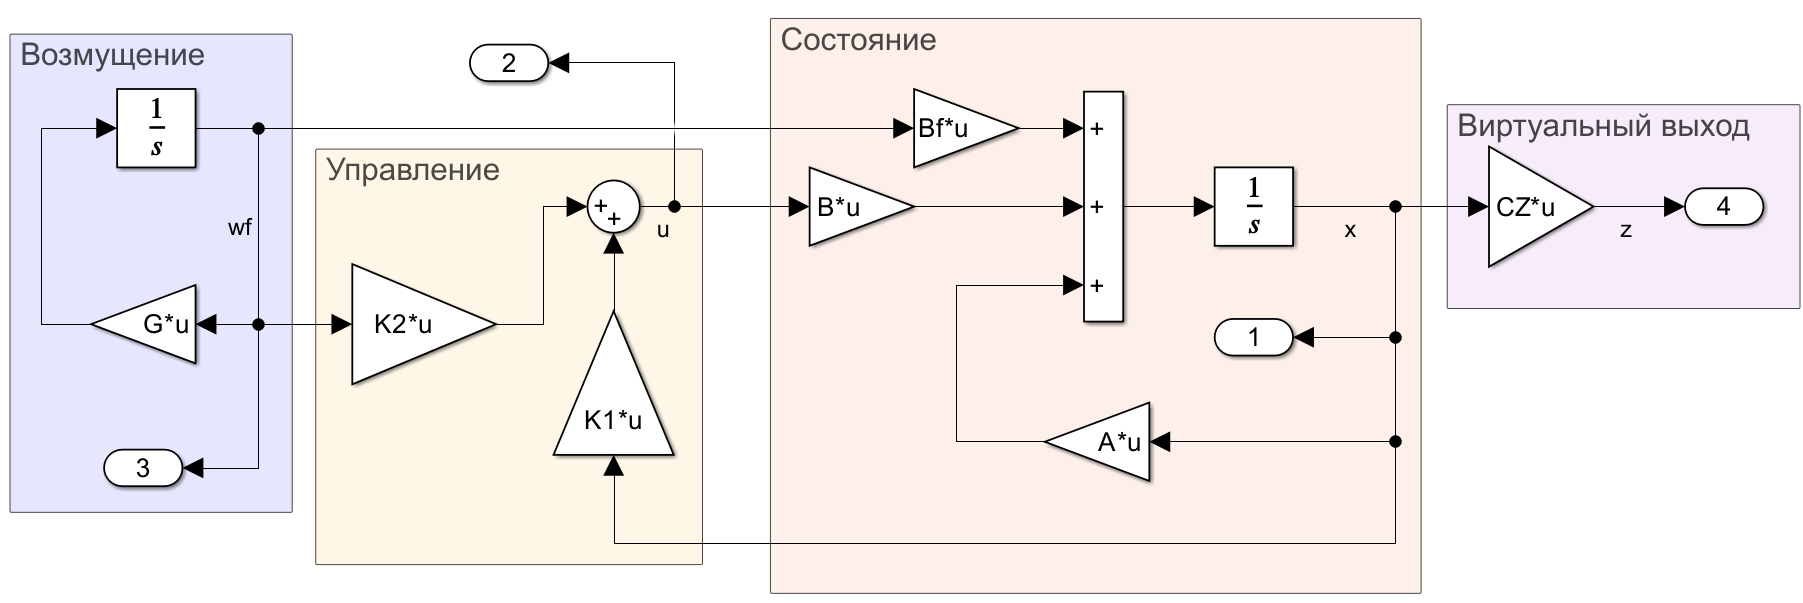
\includegraphics[width=\linewidth]{figs/task1_slx.png}
    \caption{Схема моделирования системы \eqref{eq:sys1},
    замкнутой компенсирующим регулятором \eqref{eq:reg1}}
    \label{fig:sys1}
\end{figure}

\subsection{Синтез ``feedback''-компоненты}
\label{sec:feedback1}
Синтезируем «feedback»-компоненту $K_1$ компенсирующего регулятора \eqref{eq:reg1}
с помощью уравнения Сильвестра:
\begin{equation}
    \label{eq:silv}
    AP-P\Gamma_R=BY,\quad K=-YP^{-1}.
\end{equation}
Но сначала нужно усечть систему. Найдем жордановые формы матриц:
\begin{equation*}
    A_J=\begin{bmatrix}
        -2&     0&     0\\
        0&     2&    -1\\
        0&     1&     2   
    \end{bmatrix},\quad
    B_J=\begin{bmatrix}
        0\\
        0.7071\\
       -2.1213
    \end{bmatrix},\quad
    P_J = \begin{bmatrix}
        -1&    0.7071&   -0.7071\\
        1&   -1.4142&         0\\
             0    &1.4142&         0
    \end{bmatrix},
\end{equation*}
где $P_J$ - матрица перехода. Усечем до следущих матриц:
\begin{equation*}
    A_j=\begin{bmatrix}
        2&    -1\\
        1&     2   
    \end{bmatrix},\quad
    B_j=\begin{bmatrix}
        0.7071\\
       -2.1213
    \end{bmatrix}.
\end{equation*}
возьмем следующие матрицы $\Gamma_R$ и $Y$, чтобы итоговый спект был устойчив и
пара ($\Gamma_R$, $Y$) наблюдаема
\begin{equation*}
    \Gamma_R=\begin{bmatrix}
        -10 & 1\\0&-10
    \end{bmatrix},\quad
    Y=\begin{bmatrix}
        1 & 0
    \end{bmatrix}.
\end{equation*}
Используя CVX получим следующую матрицу регулятора
\begin{equation*}
    K_{1_j}=\begin{bmatrix}
        -64.0645&-10.0410
    \end{bmatrix},
\end{equation*}
расширим и вернем в изначальный базис
\begin{equation*}
    K_1=\begin{bmatrix}
        0&K_{1_j}
    \end{bmatrix}\times P_J^{-1}=
    \begin{bmatrix}
        14.2001&	14.2001&	-38.2004
    \end{bmatrix}.
\end{equation*}
Проверим, что получили желаемый спектр
\begin{equation*}
    \sigma(A+BK_1)=\{-9.9628,\    -10.0374,\    -2.0000\}.
\end{equation*}
Регулятор найден успешно.


\subsection{Синтез ``feedforward''-компоненты}

Синтезируем «feedforward»-компоненту $K_2$ компенсирующего регулятора \eqref{eq:reg1}.
С помощью CVX решим следующую систему
\begin{equation*}
    \begin{cases}
        P\Gamma-AP=BY+B_f\\
        C_ZP=0
    \end{cases}
\end{equation*}
относительно $P$ и $Y$ и получим $K_2$
\begin{equation*}
    K_2=Y-K_1P=\begin{bmatrix}
        -616.3844	&-913.3667	&-408.5065	&751.0739
    \end{bmatrix}.
\end{equation*}

\subsection{Моделирование}
Выполним компьютерное моделирование системы. На \autoref{fig:1.1} графики
разомкнутой системы ($u=0$), по ним видно, что система неустойчива. На
\autoref{fig:1.2} сравнение системы замкнутой только ``feedback''-компонентой
и с компенсирущим регулятором \eqref{eq:reg1}. Использование только $K_1$
компоненты регулятора не смогло свести виртуальный выход к нулю как и
компенсировать возмущения в состоянии системы. 
Компенсирующий же регулятор успешно компенсировал внешнее воздействие,
сведя виртуальный выход к нулю.
\begin{figure}[H]
    \centering
    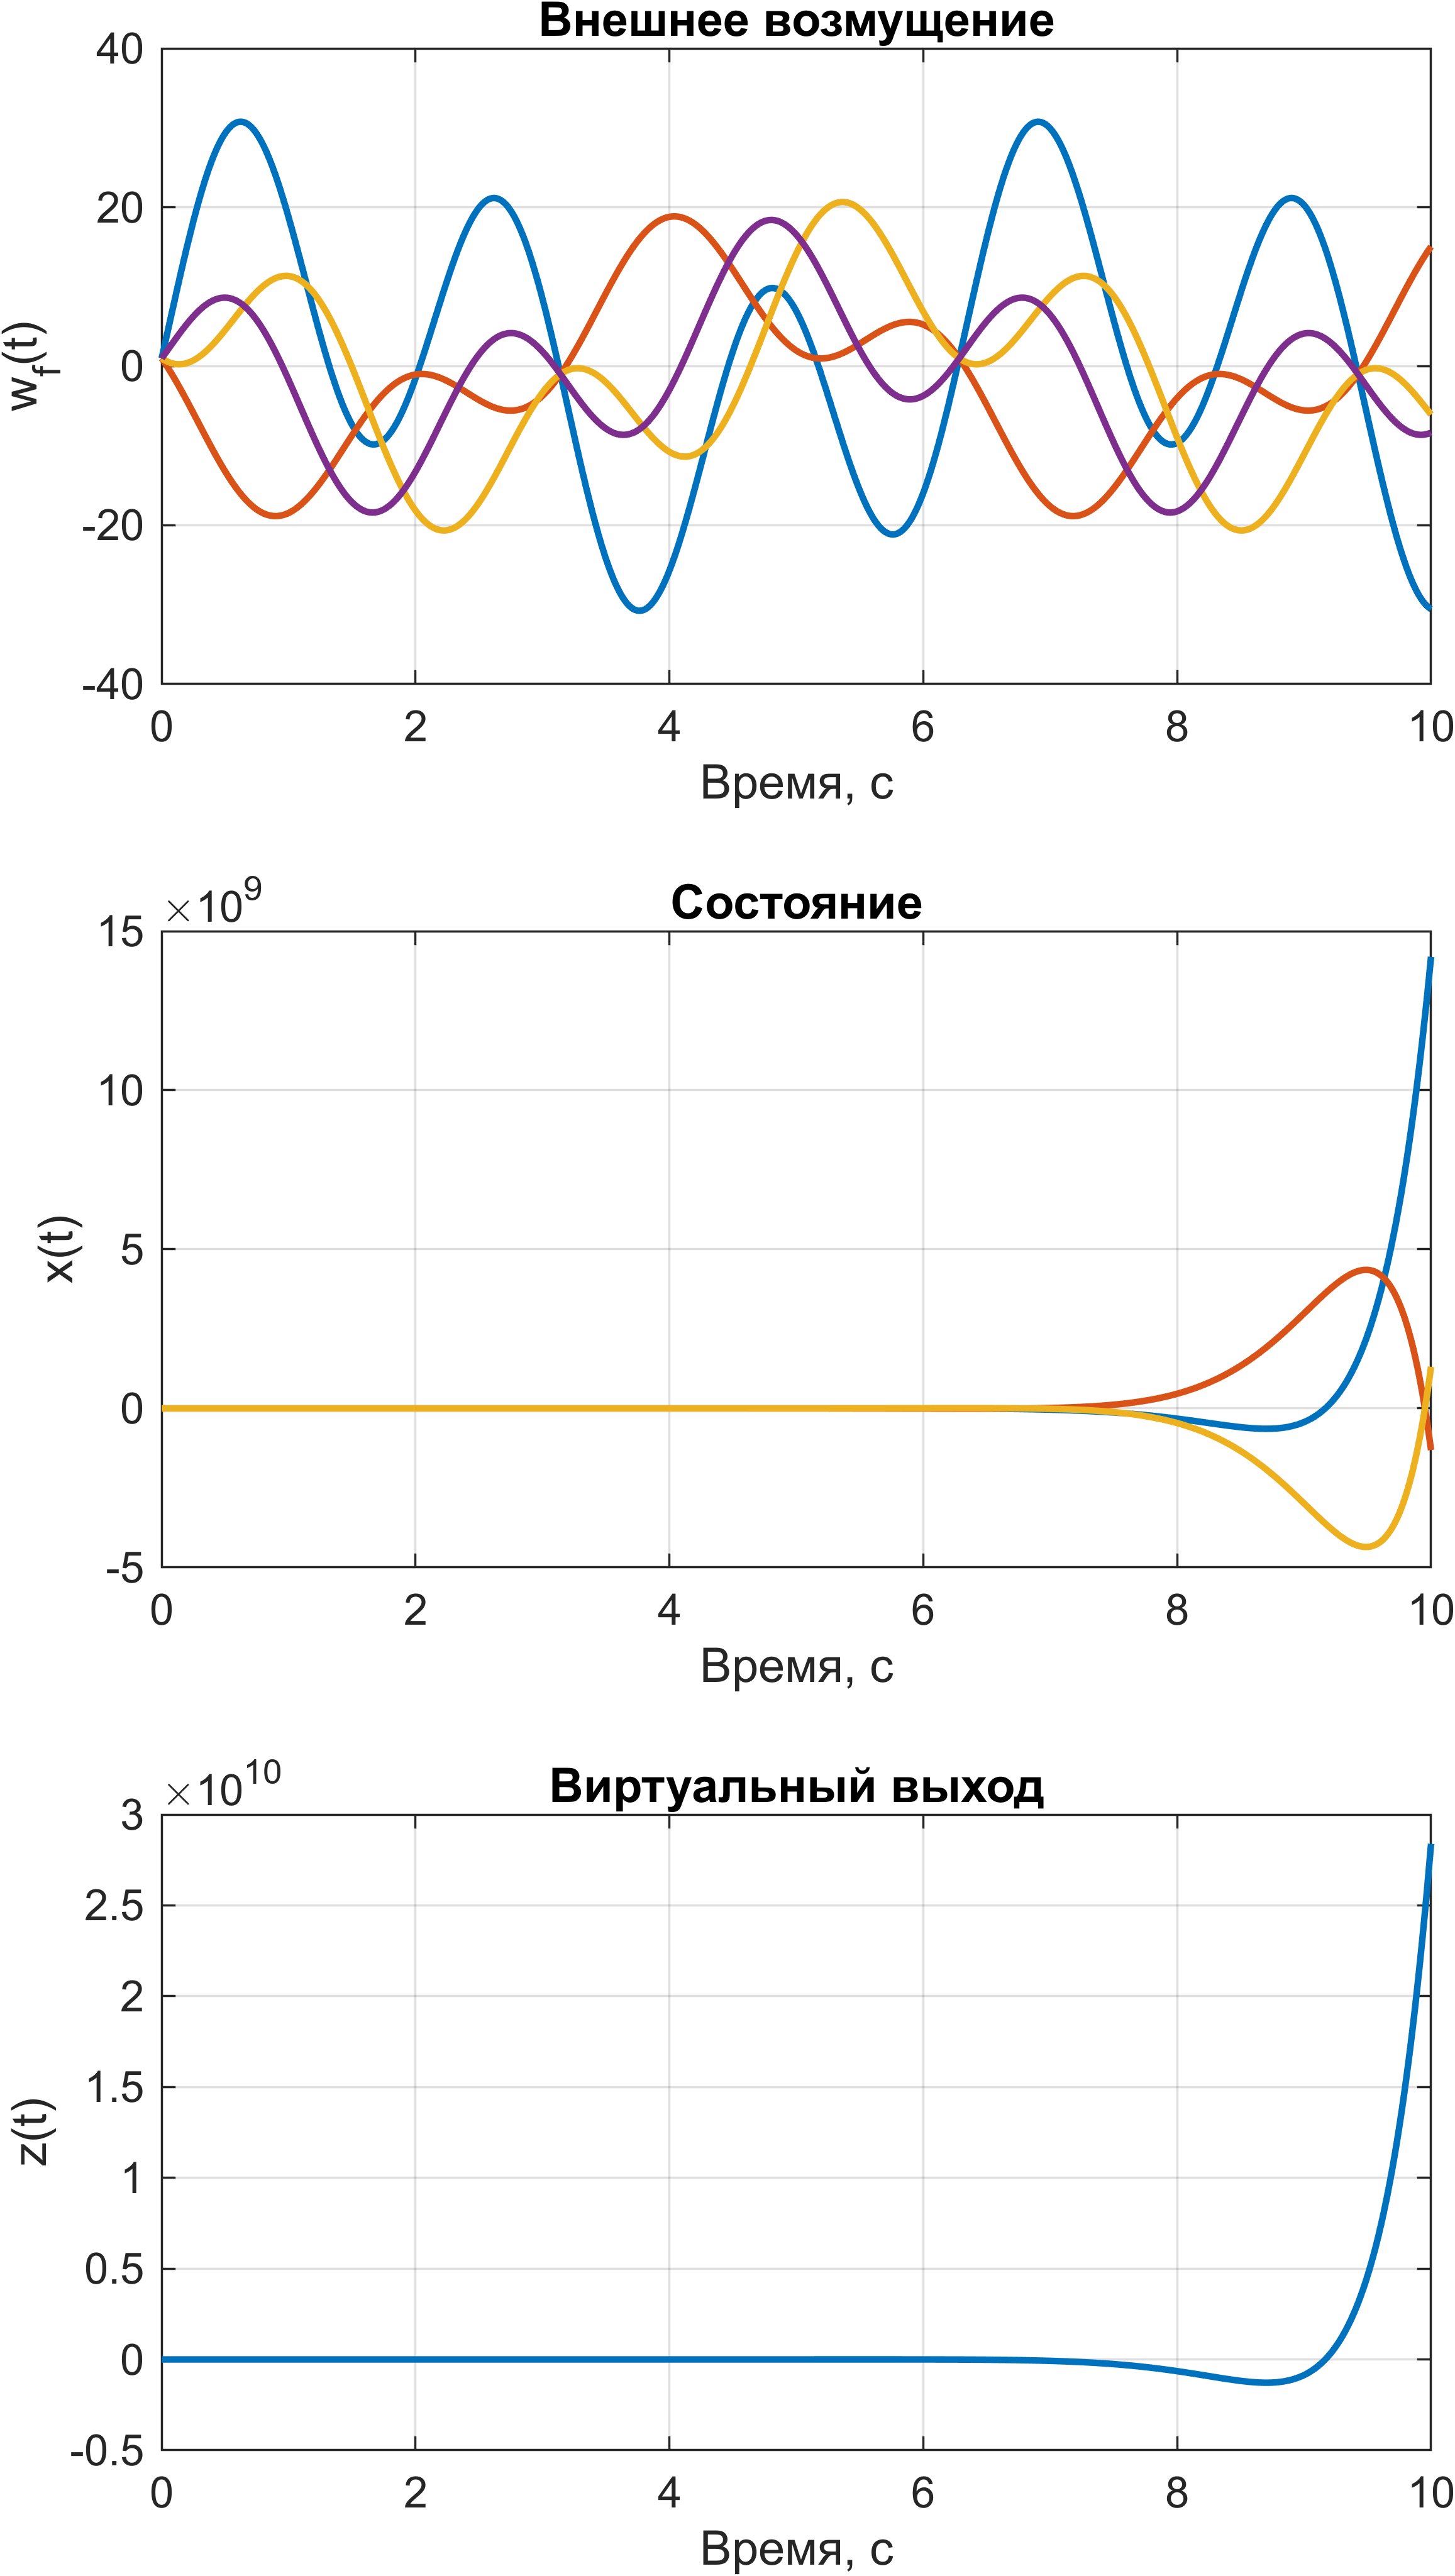
\includegraphics[width=0.8\linewidth]{figs/task1_1.png}
    \caption{Графики разомкнутой системы \eqref{eq:sys1}}
    \label{fig:1.1}
\end{figure}
\begin{figure}[H]
    \centering
    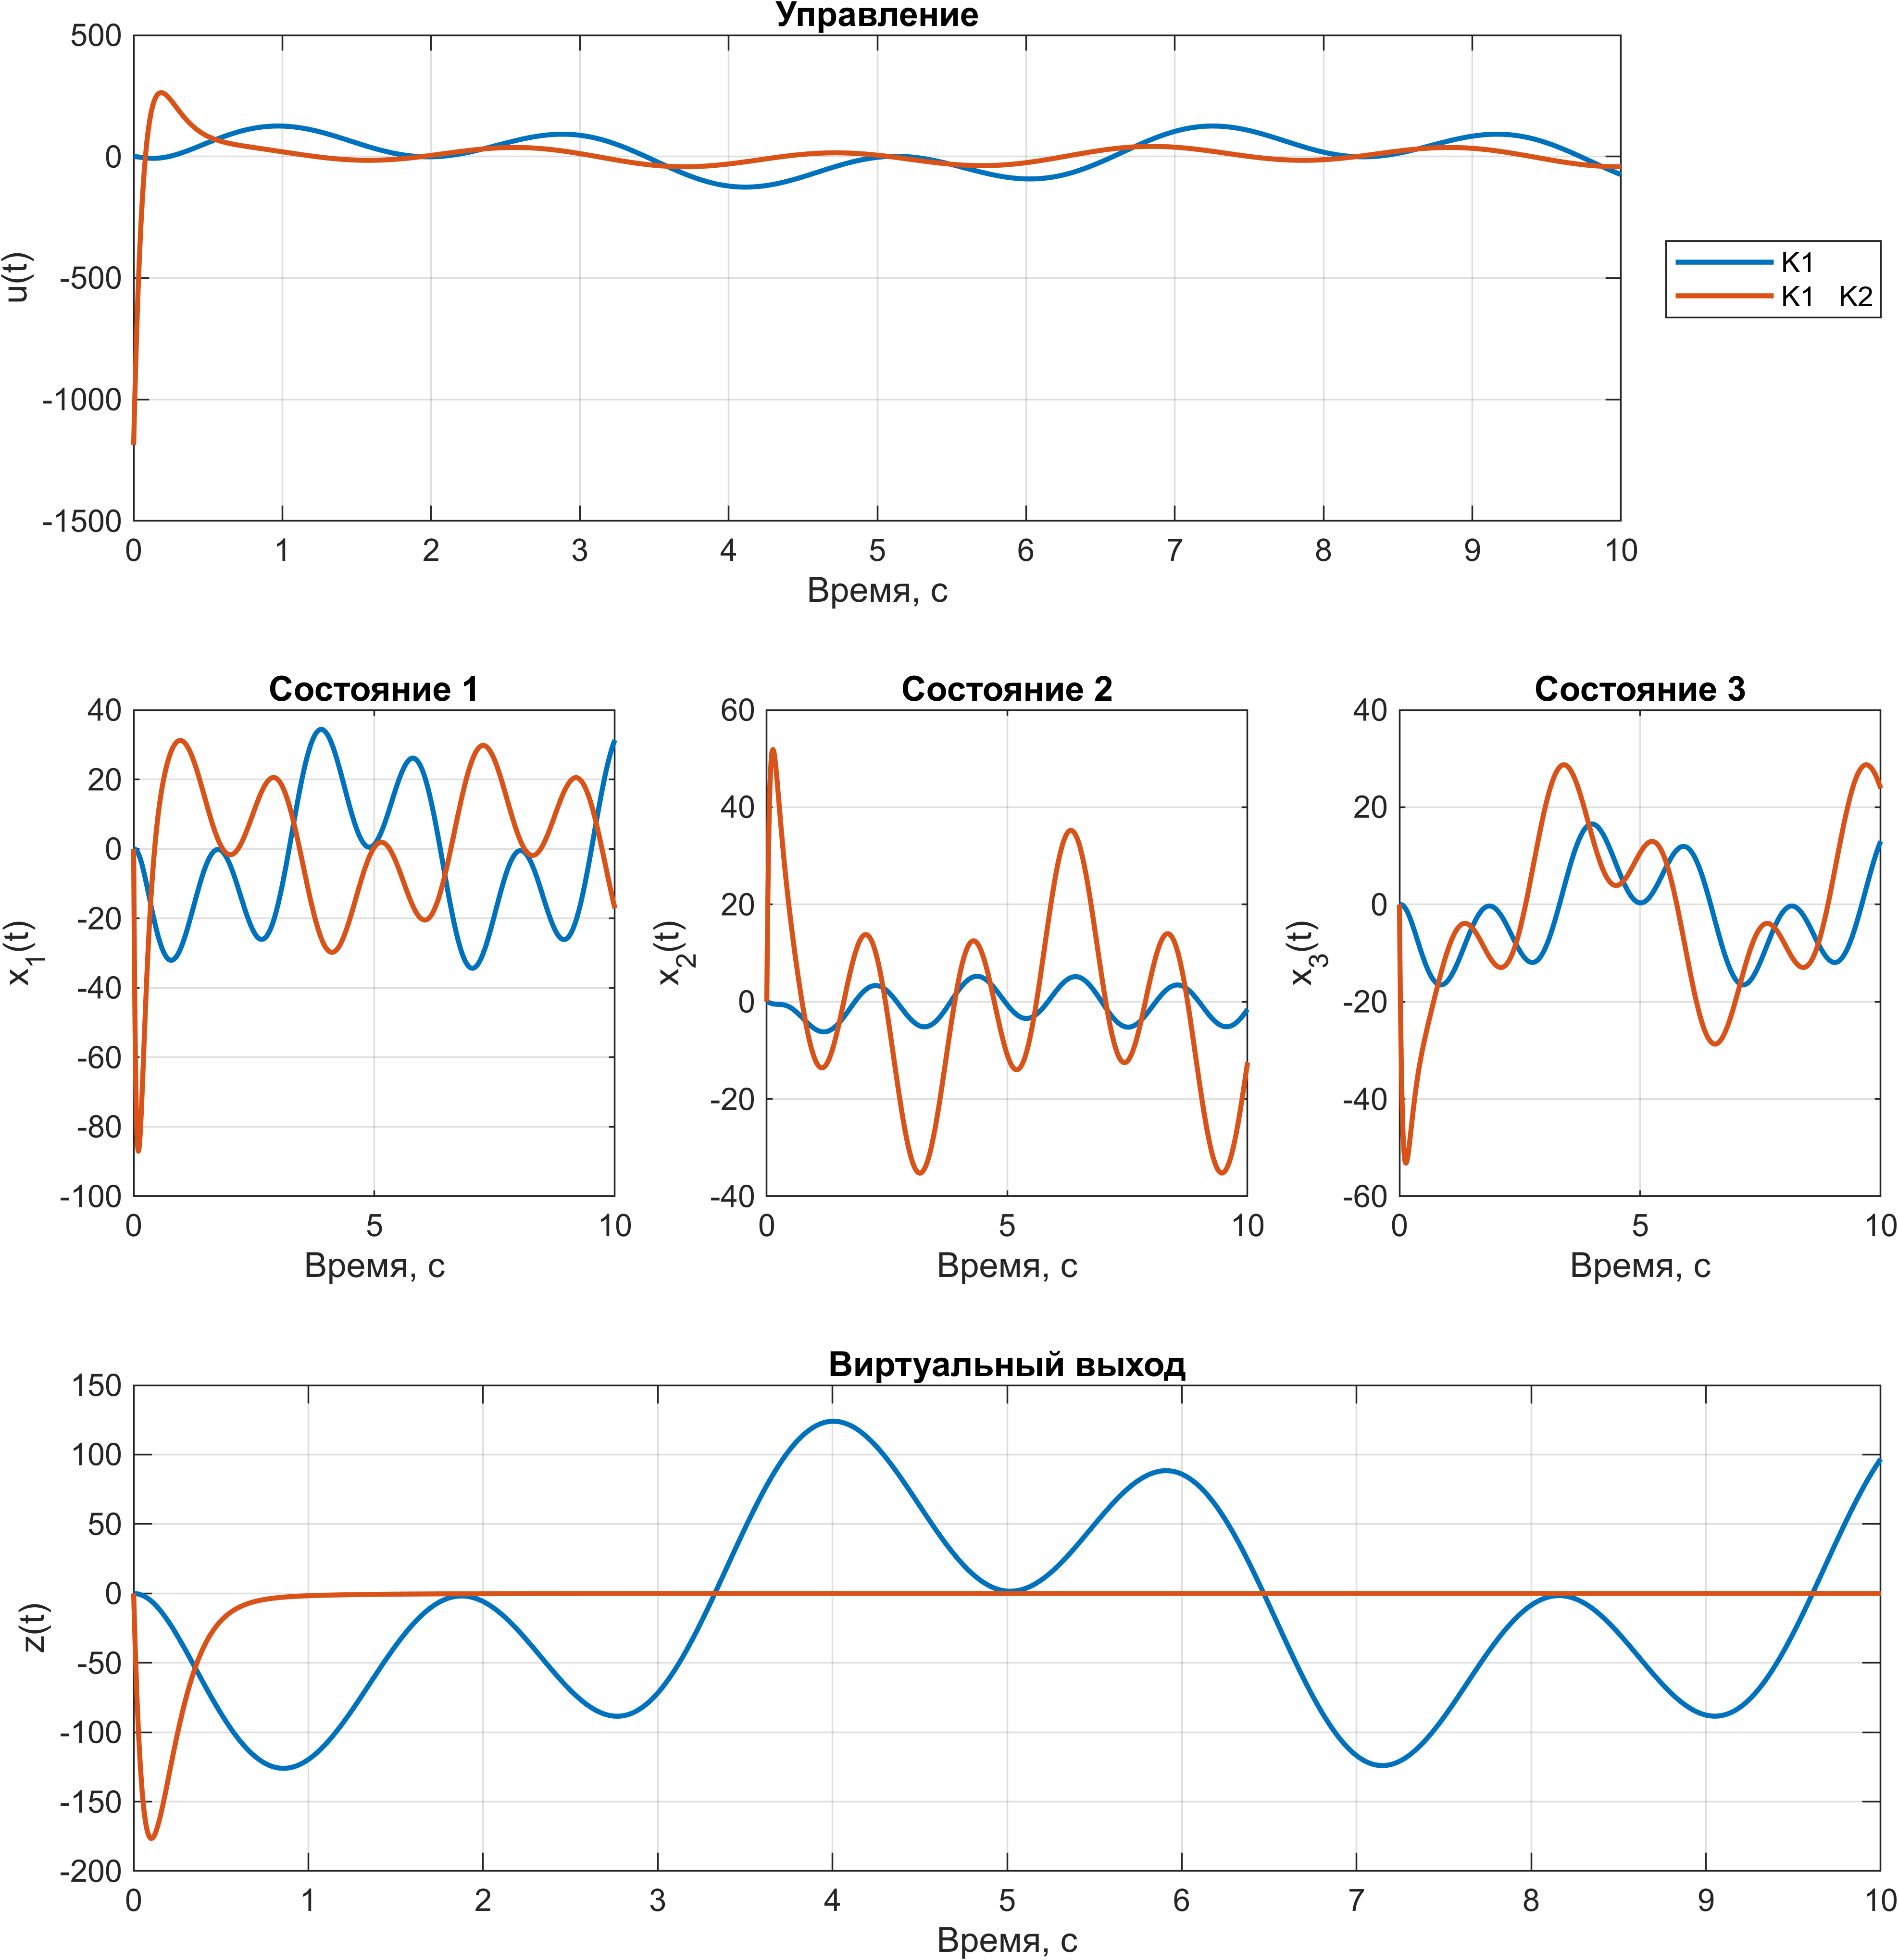
\includegraphics[width=\linewidth]{figs/task1_2.png}
    \caption{Графики замкнутой системы \eqref{eq:sys1} только с ``feedback''-компонентой
    и компенсирующим регулятором \eqref{eq:reg1}}
    \label{fig:1.2}
\end{figure}

\subsection{Вывод}

Был успешно синтезирован компенсирующий регулятор по состоянию, 
состоящий из ``feedback``- и ``feedforward``-компонент. Проведенное 
моделирование показало, что использование только ``feedback``-компоненты 
не позволяет свести виртуальный выход к нулю, тогда как полный 
компенсирующий регулятор эффективно компенсирует внешние возмущения 
и обеспечивает выполнение целевого условия.



\section{Следящий регулятор по состоянию}

\subsection{Анализ системы}
Рассмотрим систему
\begin{equation}
    \dot x=Ax+Bu,\quad x(0)=\begin{bmatrix}
        1&1&1
    \end{bmatrix}^T,
    \label{eq:sys2}
\end{equation}
генератор внешнего возмущения
\begin{equation*}
    \dot w_g=\Gamma w_g,\quad w_g(0)=\begin{bmatrix}
        1&1&1&1
    \end{bmatrix}^T
\end{equation*}
и виртуальный выход вида
\begin{equation*}
    z=C_Zx+D_Zw_g,
\end{equation*}
где
\begin{equation*}
    A=\begin{bmatrix}
        3&5&4\\
        -2&-4&-5\\
        2&2&3
    \end{bmatrix},\quad
    B=\begin{bmatrix}
        2\\-1\\1
    \end{bmatrix},\quad
    C_Z=\begin{bmatrix}
        2&3&3
    \end{bmatrix},
\end{equation*}
\begin{equation*}
    \Gamma=\begin{bmatrix}
        35&56&22&-42\\
        -11&-17&-7&12\\
        -6&-10&-5&10\\
        11&18&6&-13
    \end{bmatrix},\quad
    D_Z=\begin{bmatrix}
        3&4&2&-3
    \end{bmatrix}.
\end{equation*}
Матрица $\Gamma$ абсолютно идентична матрице из \autoref{sec:task1},
поэтому ее спектр и характер возмущения остаются прежними.
Матрицы $A$ и $B$ также не изменились, поэтому система остается
стабилизируемой. Построим схему моделирования системы \eqref{eq:sys2},
замкнутой следящим регулятором
\begin{equation}
    u=K_1x+K_2w_g.
    \label{eq:reg2}
\end{equation}
Ее можно увидеть на \autoref{fig:sys2}.
\begin{figure}[H]
    \centering
    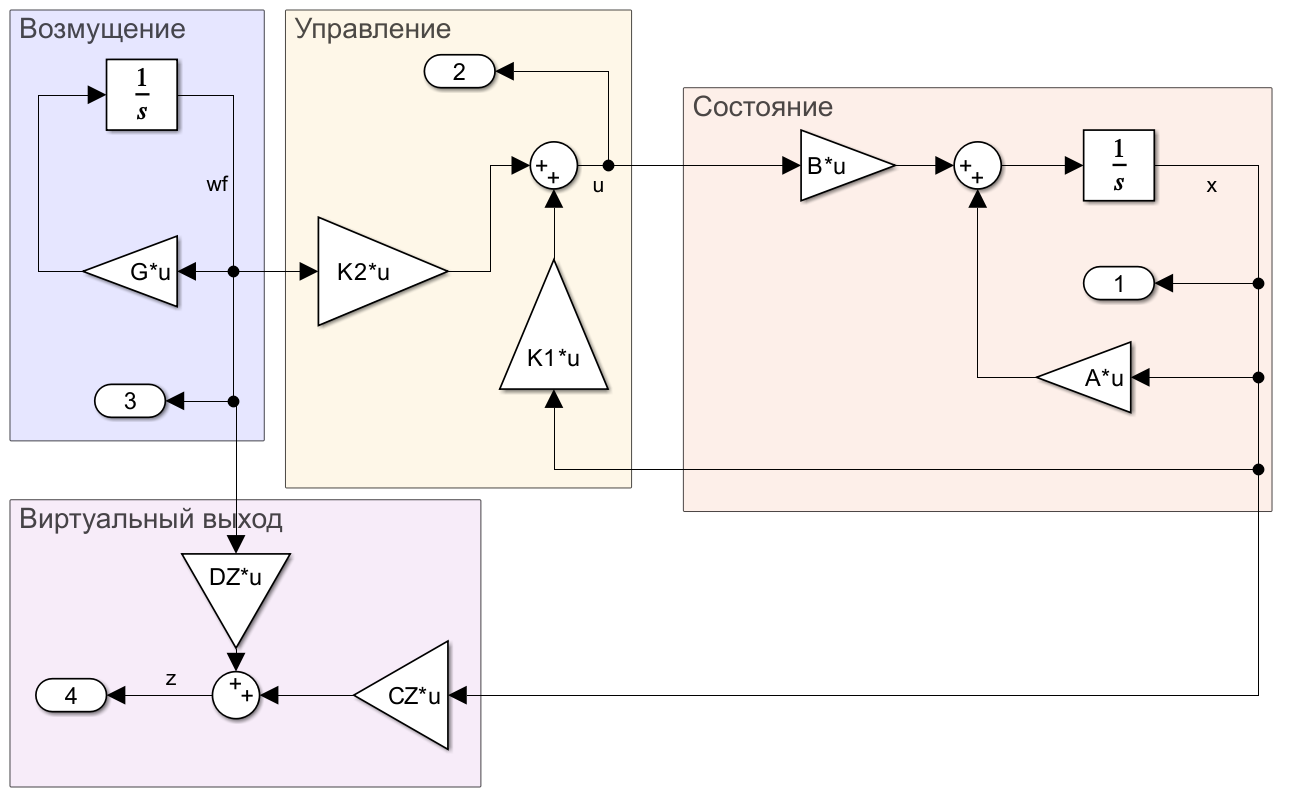
\includegraphics[width=\linewidth]{figs/task2_slx.png}
    \caption{Схема моделирования системы \eqref{eq:sys2}}
    \label{fig:sys2}
\end{figure}
Далее, синтезируем следящий регулятор по состоянию, но
``feedback''-компоненту синтезировать не нужно, возьмем
ее из \autoref{sec:feedback1}, она подойдет, так как
пара ($A$, $B$) не изменилась.

\subsection{Синтез ``feedforward''-компоненты}

Синтезируем «feedforward»-компоненту $K_2$ следящего регулятора \eqref{eq:reg2}.
С помощью CVX решим следующую систему
\begin{equation*}
    \begin{cases}
        P\Gamma-AP=BY\\
        C_ZP+D_Z=0
    \end{cases}
\end{equation*}
относительно $P$ и $Y$ и получим $K_2$
\begin{equation*}
    K_2=Y-K_1P=\begin{bmatrix}
        90.7624&	145.6219&	64.7442&	-109.6806
    \end{bmatrix}.
\end{equation*}

\subsection{Моделирование}
Выполним компьютерное моделирование системы. На \autoref{fig:2.1} графики
разомкнутой системы ($u=0$), по ним видно, что система неустойчива. На
\autoref{fig:2.2} сравнение системы замкнутой только ``feedback''-компонентой
и с компенсирущим регулятором \eqref{eq:reg2}. Использование только $K_1$
компоненты регулятора не смогло свести виртуальный выход к нулю (проследить за 
возмущающим сигналом), но система стала асимптотически устойчивой. 
Компенсирующий же регулятор успешно проследил за возмущением,
сведя виртуальный выход к нулю.
\begin{figure}[H]
    \centering
    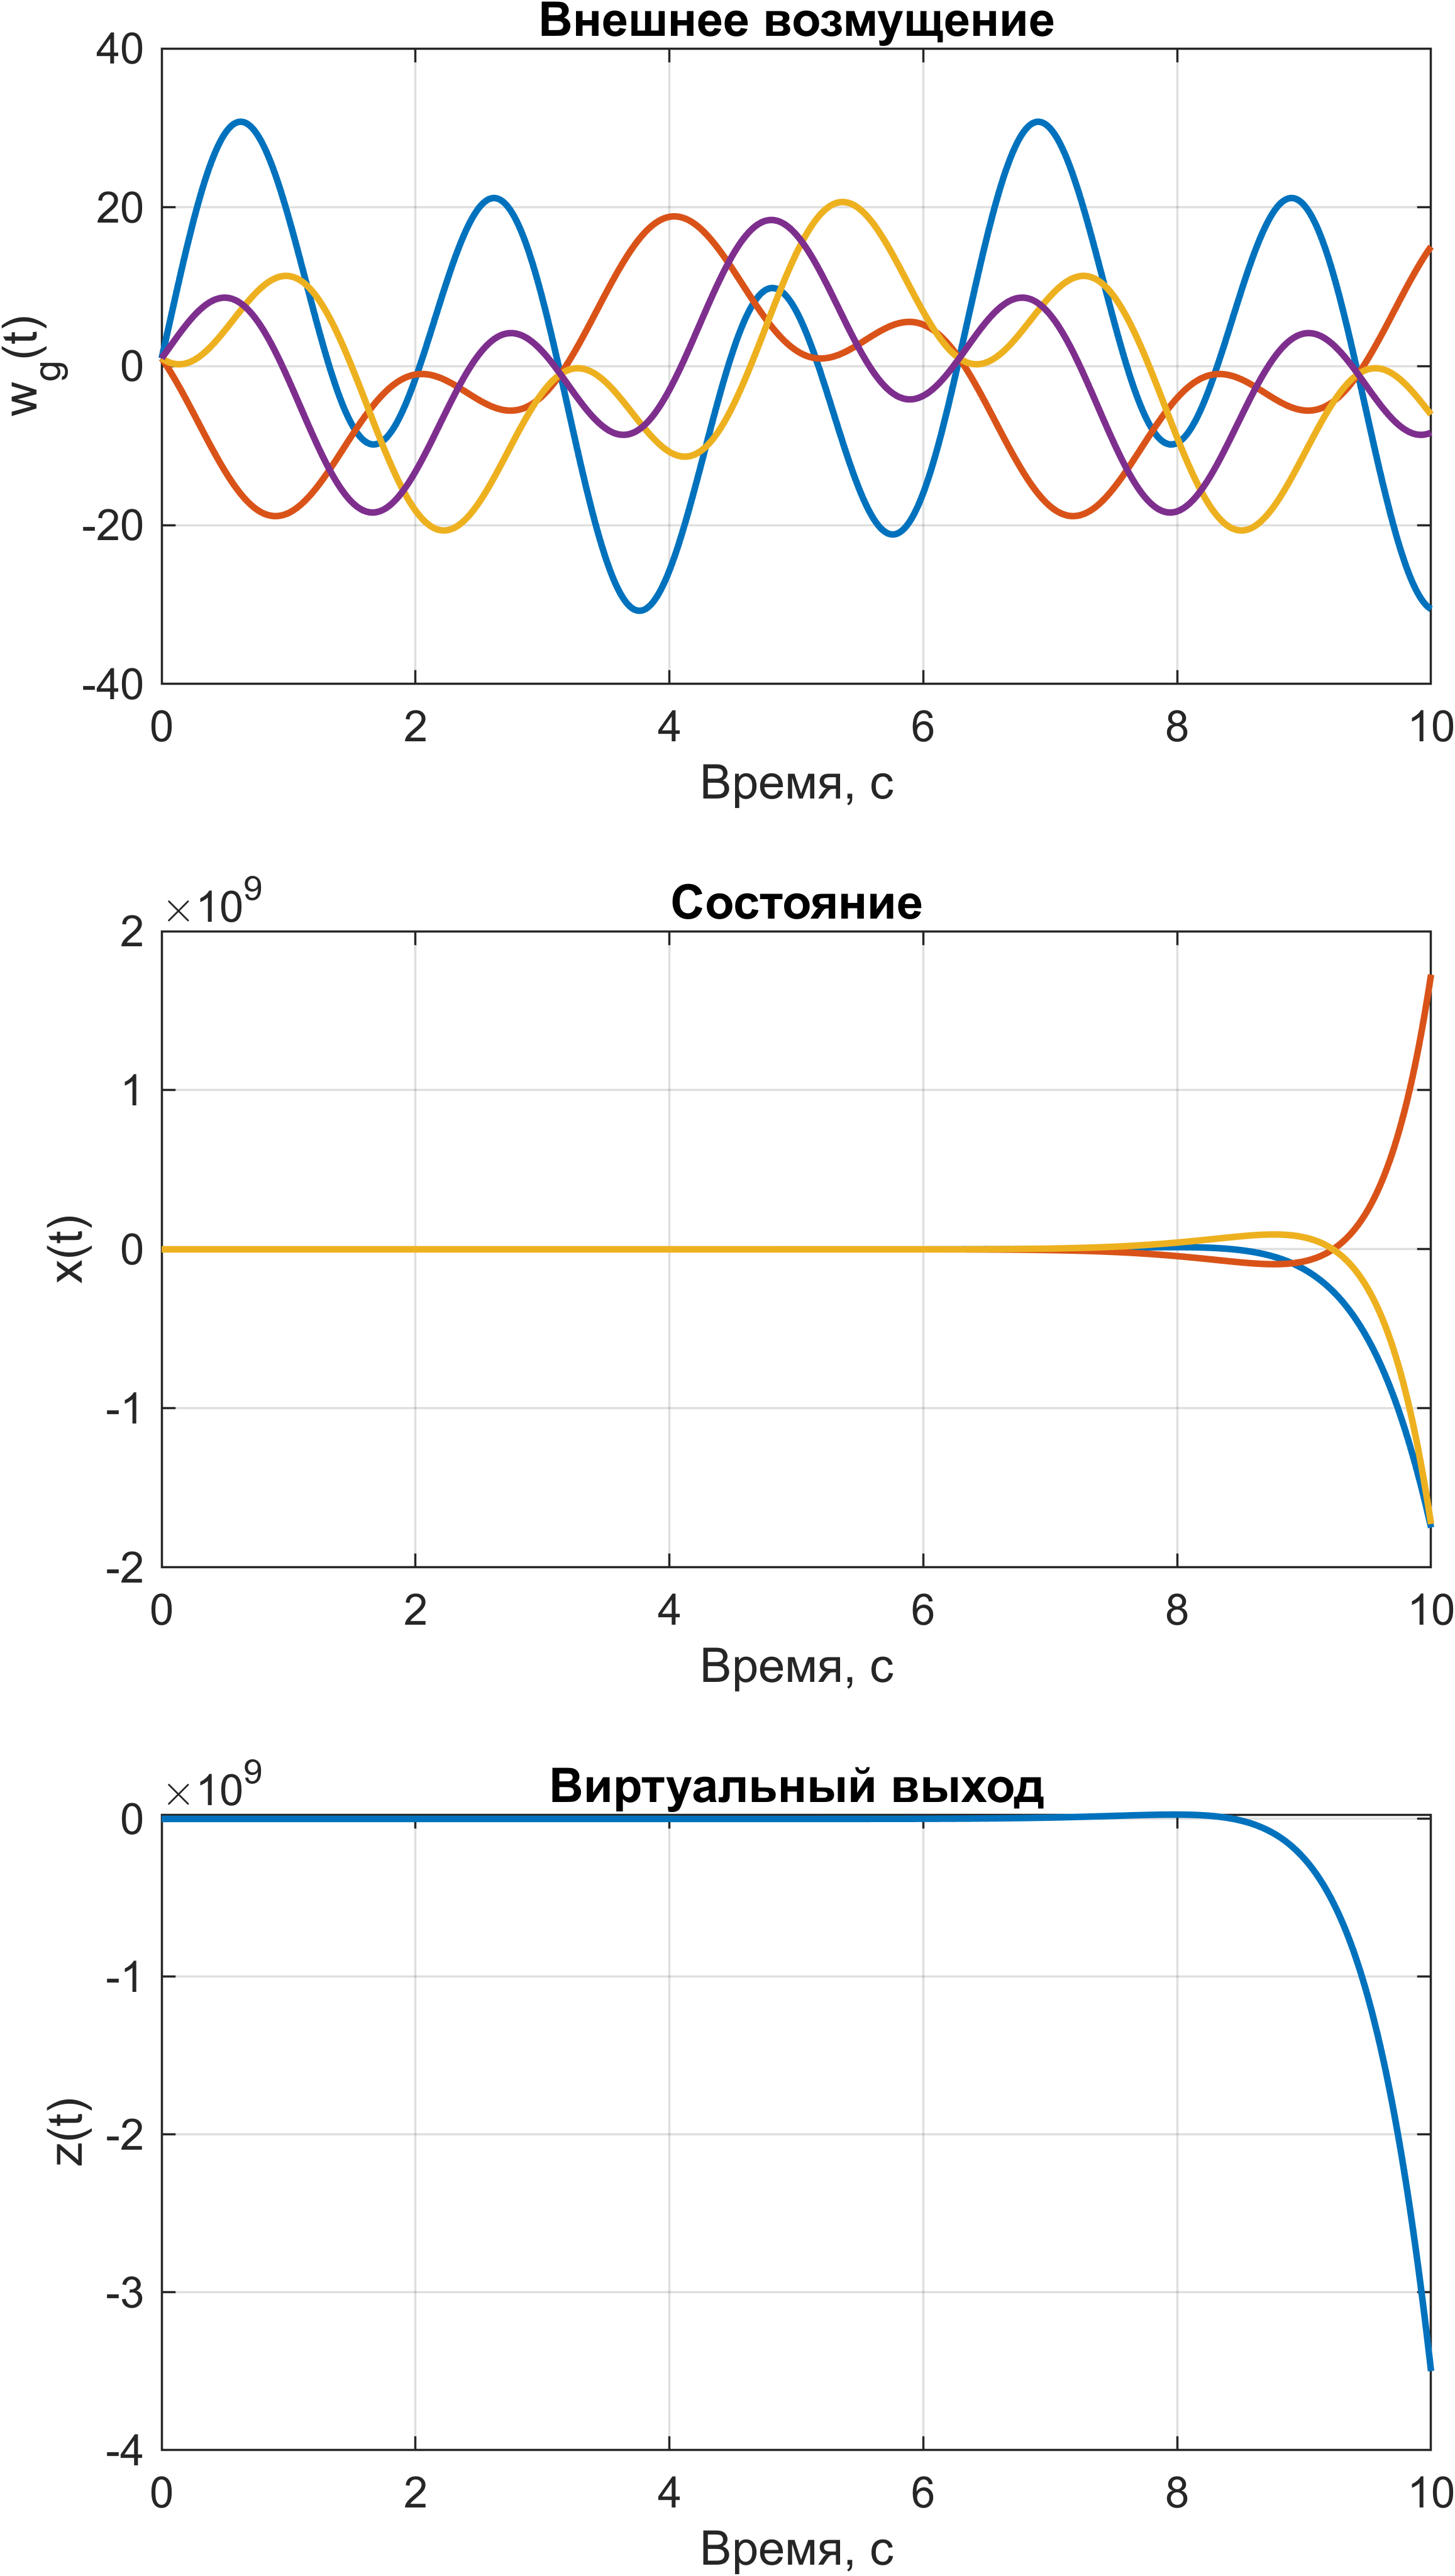
\includegraphics[width=0.8\linewidth]{figs/task2_1.png}
    \caption{Графики разомкнутой системы \eqref{eq:sys2}}
    \label{fig:2.1}
\end{figure}
\begin{figure}[H]
    \centering
    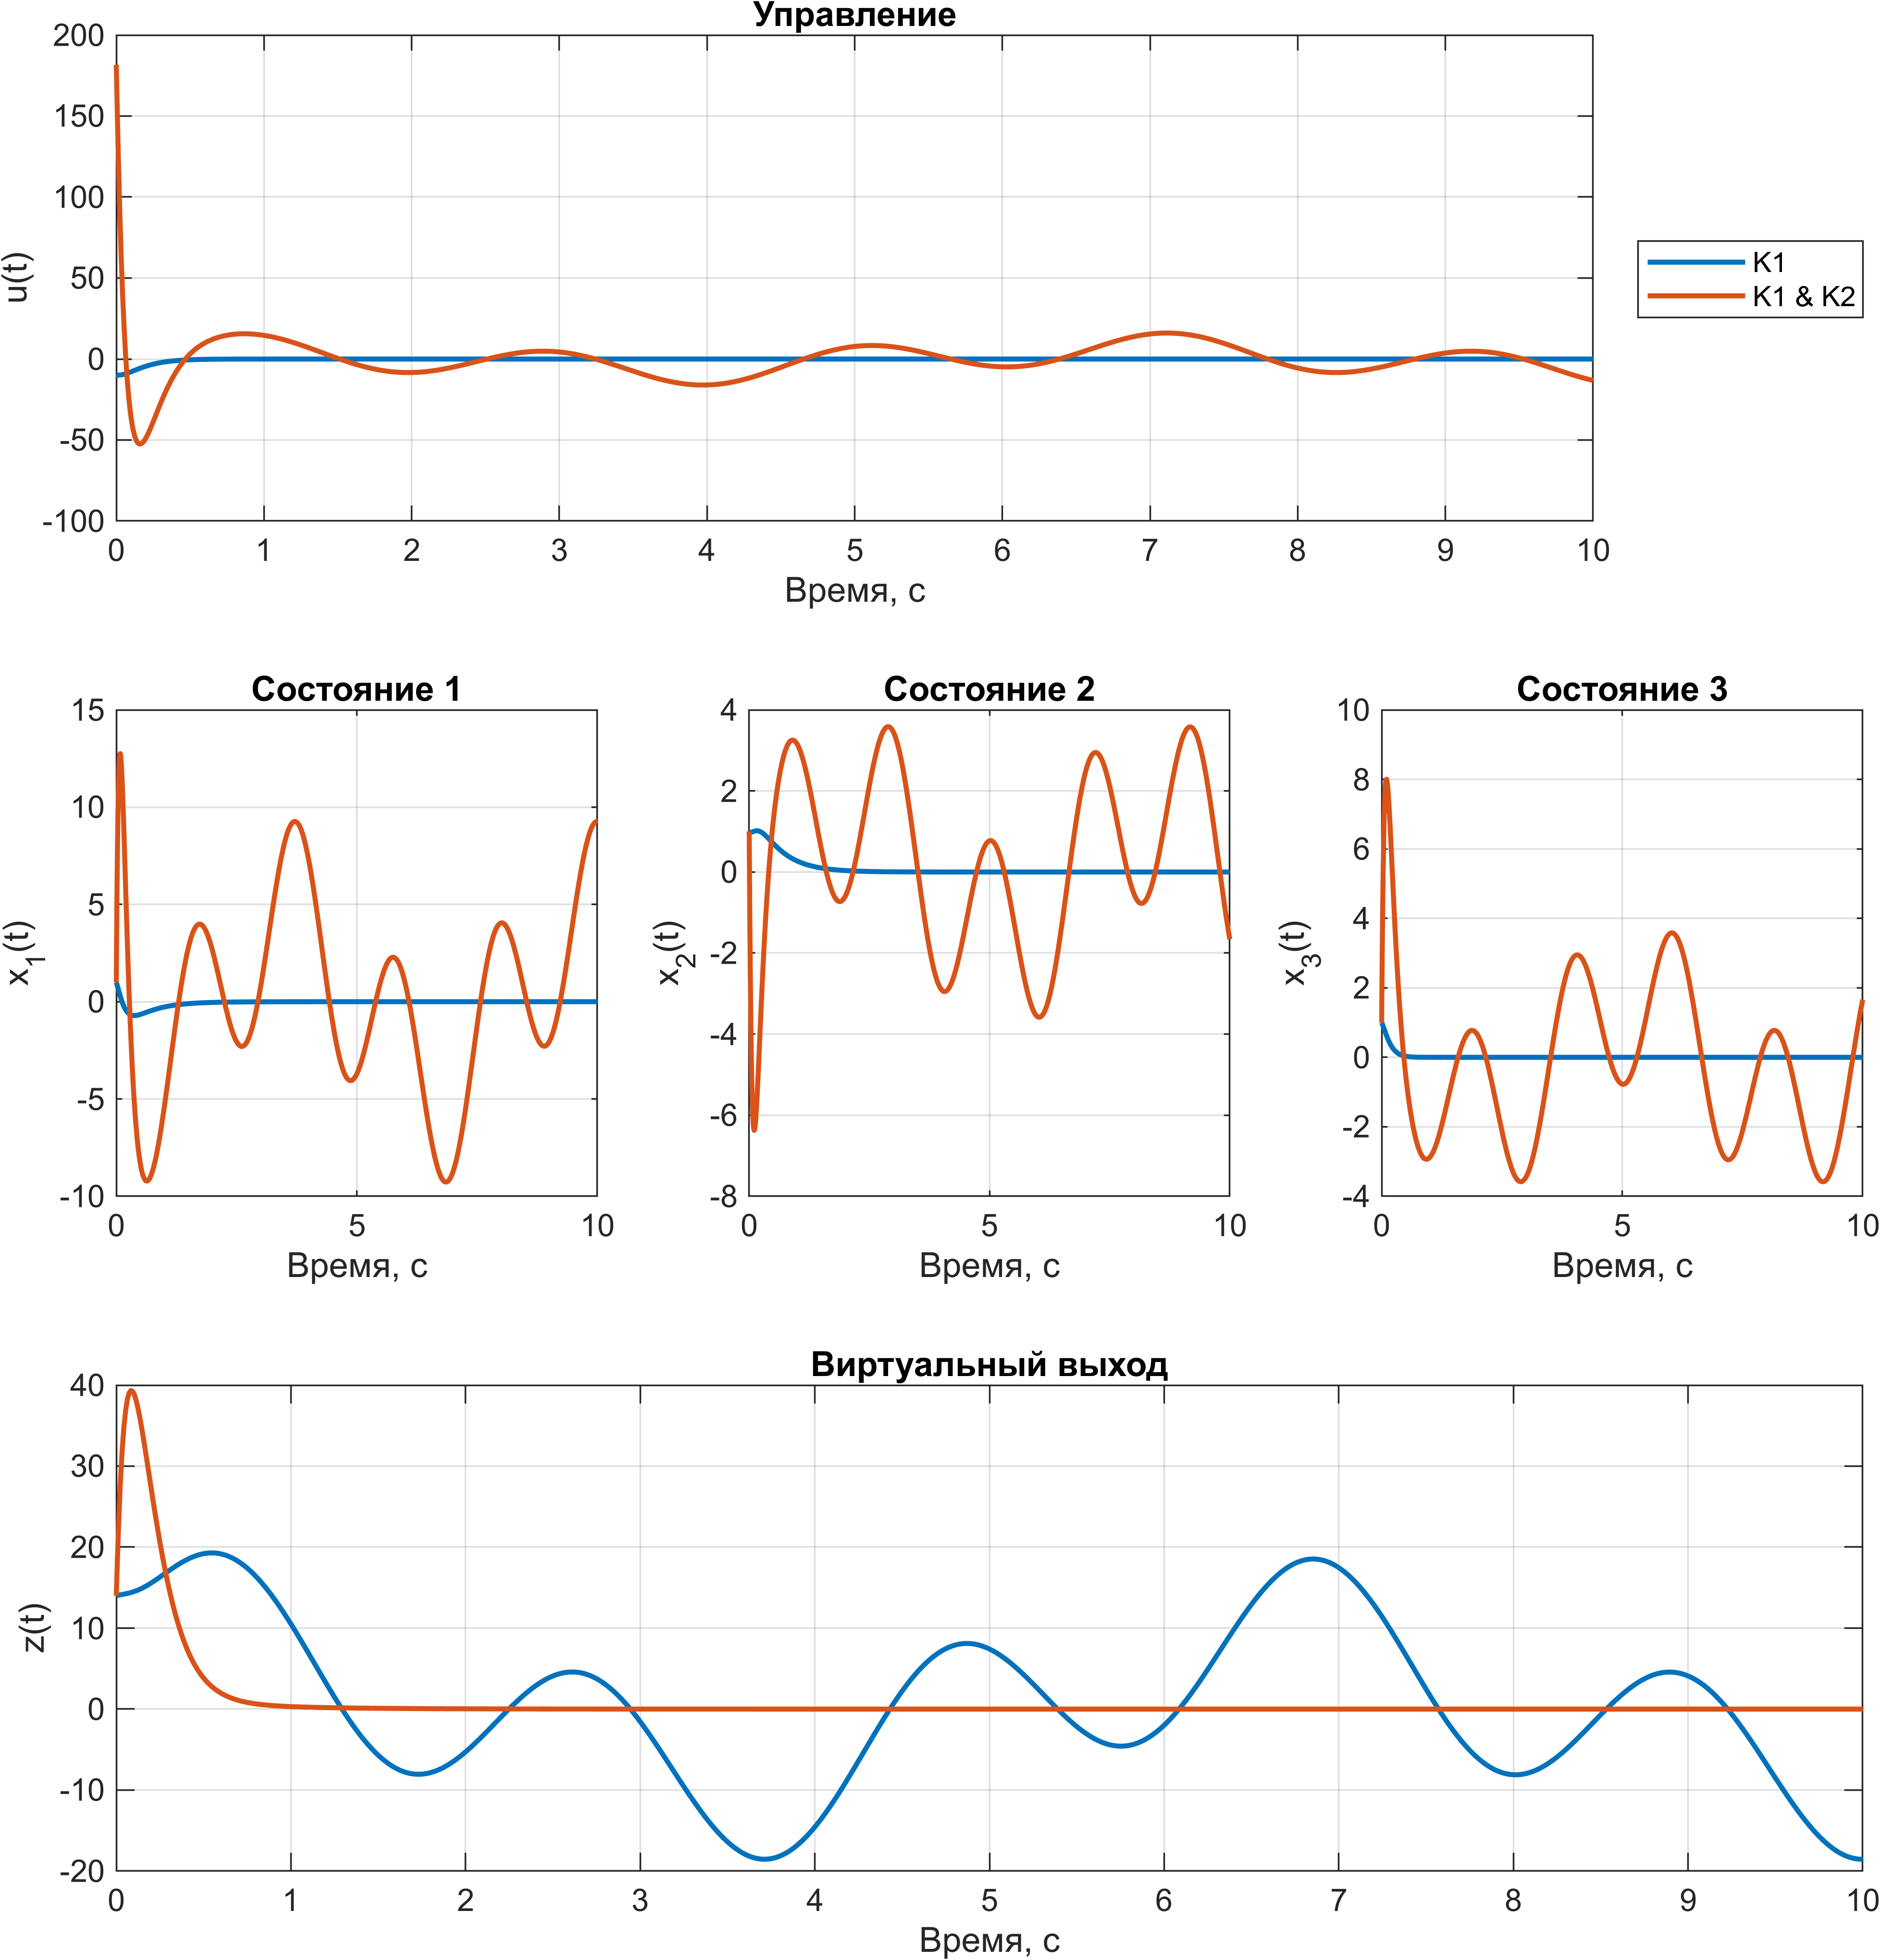
\includegraphics[width=\linewidth]{figs/task2_2.png}
    \caption{Графики замкнутой системы \eqref{eq:sys2} только с ``feedback''-компонентой
    и с компенсирующим регулятором \eqref{eq:reg2}}
    \label{fig:2.2}
\end{figure}

\subsection{Вывод}

Был успешно синтезирован следящий регулятор по состоянию, состоящий 
из ``feedback``- и ``feedforward``-компонент. Проведенное моделирование 
показало, что использование только ``feedback``-компоненты делает 
систему асимптотически устойчивой, но не позволяет свести виртуальный 
выход к нулю. Полный следящий регулятор успешно следит за внешним
возмущением и обеспечивает выполнение целевого условия.


\newpage
\section{Слежение и компенсация по выходу}
\subsection{Анализ системы}
Рассмотрим систему
\begin{equation}
    \begin{cases}
        \dot x=Ax+Bu+B_fw,\\
        y=Cx+Dw,
    \end{cases}\quad
    x(0)=\begin{bmatrix}
        0&0&0
    \end{bmatrix}^T,
    \label{eq:sys3}
\end{equation}
и генератор внешнего воздействия
\begin{equation*}
    \dot w=\Gamma w,\quad w(0)=\begin{bmatrix}
        1&1&1&1
    \end{bmatrix}^T,
\end{equation*}
где
\begin{equation*}
    A=\begin{bmatrix}
        3&5&4\\
        -2&-4&-5\\
        2&2&3
    \end{bmatrix},\quad
    B=\begin{bmatrix}
        2\\-1\\1
    \end{bmatrix},\quad
    B_f=\begin{bmatrix}
        -2&0&0&2\\
        -2&0&0&0\\
        0&0&0&0
    \end{bmatrix},
\end{equation*}
\begin{equation*}
    C=\begin{bmatrix}
        -2&-1&0
    \end{bmatrix},\quad
    D=\begin{bmatrix}
        1&2&1&-1
    \end{bmatrix},
\end{equation*}
\begin{equation*}
    \Gamma=\begin{bmatrix}
        35&56&22&-42\\
        -11&-17&-7&12\\
        -6&-10&-5&10\\
        11&18&6&-13
    \end{bmatrix}.
\end{equation*}
Матрица $\Gamma$ абсолютно идентична матрице из \autoref{sec:task1},
поэтому ее спектр и характер возмущения остаются прежними. Для
управляемости по выходу необходимо, чтобы пара 
\begin{equation*}
   c=
    \begin{bmatrix}
        -2\\	-1\\	0\\	1\\	2\\	1\\	-1
    \end{bmatrix}^T,\quad
    \begin{bmatrix}
        A&B_f\\0&\Gamma
    \end{bmatrix}=
    \begin{bmatrix}
        3  &  5  &  4  & -2  &  0  &  0  &  2  \\
           -2  & -4  & -5  & -2  &  0  &  0  &  0  \\
        2  &  2  &  3  &  0  &  0  &  0  &  0  \\
        0  &  0  &  0  & 35  & 56  & 22  & -42 \\
        0  &  0  &  0  & -11 & -17 & -7  &  12 \\
        0  &  0  &  0  & -6  & -10 & -5  &  10 \\
        0  &  0  &  0  & 11  & 18  &  6  & -13
    \end{bmatrix}
\end{equation*}
была обнаружимаема. Используя матрицу наблюдаемости
\begin{equation*}
    V=\begin{bmatrix}
        -2   & -1   &  0   &  1   &  2   &  1   & -1 \\
        -4   & -6   & -3   &  2   & -6   & -3   &  1 \\
        -6   & -2   &  5   & 185  & 262  & 107  & -207 \\
        -4   & -12  &  1   & 690  & 1110 & 459  & -877 \\
        14   & 30   & 47   & -429 & -606 & -147 & 323 \\
        76   & 44   & 47   & -4002 & -6438 & -2523 & 5105 \\
        234  & 298  & 225  & 1801 & 2454 & 267  & -615
    \end{bmatrix},
\end{equation*}
можно убедиться, что система полность наблюдаема
($rank\ V = 7$), а значит и обнаруживаема, что нужно для синтеза
наблюдателя. А так как пара ($A$, $B$) остается стабилизируемой (см. \autoref{sec:task1}),
можно успешно осуществить слежение и компенсацию по выходу с помощью наблюдателя и регулятора
\begin{equation}
    u=K_1\hat x+K_2\hat w.
    \label{eq:reg3}
\end{equation}
Построим схему моделирования системы \eqref{eq:sys3},
замкнутой регулятором \eqref{eq:reg3} и наблюдателем
\begin{equation}
    \label{eq:obs3}
    \begin{bmatrix}
        \dot{\hat x}\\
        \dot{\hat w}
    \end{bmatrix}=
    \bar A\begin{bmatrix}
        \hat x\\
        \hat w
    \end{bmatrix}
    -Ly.
\end{equation}
Для начала определим матрицы $\bar A$ и $L$ из системы полного 
наблюдателя и регулятора \eqref{eq:reg3}:
\begin{equation*}
    \begin{cases}
        \dot{\hat x}=\bar Ax+\hat Bu+\hat B_fw+L_1(\hat y-y)\\
        \dot{\hat w}=\Gamma\hat w+L_2(\hat y-y)\\
        \hat y=C\hat x+D\hat w
    \end{cases},
\end{equation*}
получим
\begin{equation*}
    \begin{cases}
        \dot{\hat x}=(A+BK_1+L_1C)\hat x+(B_f+BK_2+L_1D)\hat w-L_1y\\
        \dot{\hat w}=L_2C\hat x+(L_2D+\Gamma)\hat w-L_2y\\
    \end{cases},
\end{equation*}
тогда
\begin{equation}
    \label{eq:al}
    \bar A=\begin{bmatrix}
        A+BK_1+L_1C & B_f+BK_2+L_1D\\
        L_2C & L_2D+\Gamma
    \end{bmatrix},\quad
    L=\begin{bmatrix}
        L_1\\L_2
    \end{bmatrix}.
\end{equation}
Схему можно увидеть на \autoref{fig:sys3}.
\begin{figure}[H]
    \centering
    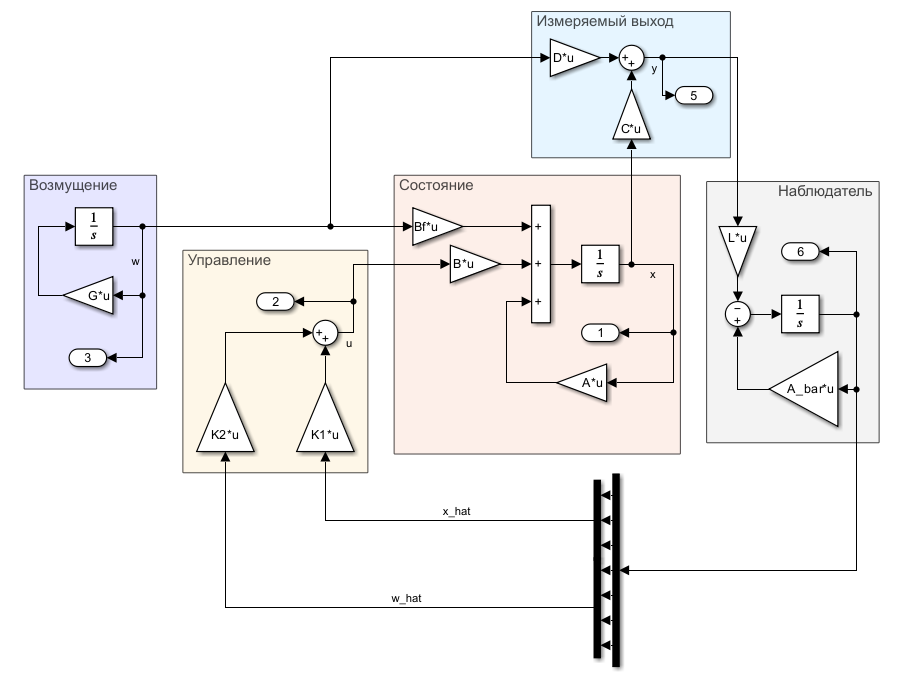
\includegraphics[width=\linewidth]{figs/task3_slx.png}
    \caption{Схема моделирования системы \eqref{eq:sys3}
    замкнутой регулятором \eqref{eq:reg3} и состоящей
    из расширенного наблюдателя \eqref{eq:obs3}}
    \label{fig:sys3}
\end{figure}
Далее, синтезируем регулятор \eqref{eq:reg3}. $K_1$ возьмем из \autoref{sec:feedback1}.


\subsection{Синтез матрицы коррекции наблюдателя}

Синтезируем матрицу коррекции $L$ наблюдателя \eqref{eq:obs3}.
Воспользуесямся уравнением Сильвестра:
\begin{equation*}
    \Gamma_OQ-QA_O=YC_O,\quad L=Q^{-1}Y.
\end{equation*}
Матрица $\Gamma_O$ доложна быть Гурвицева и
\begin{equation}
    \label{eq:cond1}
    \sigma(A_O)\cap\sigma(\Gamma_O)=\varnothing,
\end{equation}
\begin{equation}
    \label{eq:cond2}
    (\Gamma_O,\ Y) - \text{управляема},
\end{equation}
\begin{equation}
    \label{eq:cond3}
    (C_O,\ A_O)=\left( 
        \begin{bmatrix}
            C&D
        \end{bmatrix},\ 
        \begin{bmatrix}
            A&B_f\\0&\Gamma
        \end{bmatrix}
     \right) - \text{наблюдаема}.
\end{equation}
Условие \eqref{eq:cond3} уже выполнено, подберем матрицы $\Gamma_O$ и $Y$,
чтобы выполнять остальные условия:
\begin{equation*}
    \Gamma_O=\begin{bmatrix}
        -10 &  1  &  0  &  0  &  0  &  0  &  0 \\
         0  & -10 &  1  &  0  &  0  &  0  &  0 \\
         0  &  0  & -10 &  1  &  0  &  0  &  0 \\
         0  &  0  &  0  & -10 &  1  &  0  &  0 \\
         0  &  0  &  0  &  0  & -10 &  1  &  0 \\
         0  &  0  &  0  &  0  &  0  & -10 &  1 \\
         0  &  0  &  0  &  0  &  0  &  0  & -10
    \end{bmatrix},\quad
    Y=\begin{bmatrix}
         0 \\
         0 \\
         0 \\
         0 \\
         0 \\
         0 \\
         1
    \end{bmatrix}.
\end{equation*}
С помощью CVX найдем решение и получим матрицу коррекции:
\begin{equation*}
    L=\begin{bmatrix}
        -61613 &
        119150 &
        -127060 &
        11806 &
        -14420 &
        6092 &
        -6797
    \end{bmatrix}^T.
\end{equation*}


\subsection{Первый случай виртуального выхода}

Рассмотрим виртуальный выход вида:
\begin{equation*}
    z=C_Zx+D_Zw,
\end{equation*}
где
\begin{equation*}
    C_Z=\begin{bmatrix}
        2&3&3
    \end{bmatrix},\quad
    D_Z=\begin{bmatrix}
        3&4&2&-3
    \end{bmatrix}.
\end{equation*}

\subsubsection{Синтез ``feedforward''-компоненты}
Синтезируем «feedforward»-компоненту $K_2$ регулятора \eqref{eq:reg3}.
Для этого нужно решить систему уравнений
\begin{equation}
    \label{eq:getk2}
    \begin{cases}
        P\Gamma-AP=BY+B_f\\
        C_ZP+D_Z=0
    \end{cases}
\end{equation}
относительно $P$ и $Y$. Сделаем это с помощью CVX и получим
\begin{equation*}
    K_2=Y-K_1P=\begin{bmatrix}
        -525.6221&	-767.7450	&-343.7623	&641.3935
    \end{bmatrix}.
\end{equation*}

\subsubsection{Моделирование}

Выполним компьютерное моделирование замкнутой системы с нулевыми
начальными условиями наблюдателя. График формируемого регулятором 
управления $u(t)$, сравнительные графики
$\begin{bmatrix}
    x(t)\\w(t)
\end{bmatrix}$ и
$\begin{bmatrix}
    \hat x(t)\\\hat w(t)
\end{bmatrix}$, 
график ошибки наблюдателя $e(t)=\begin{bmatrix}
    x(t)\\w(t)
\end{bmatrix} - \begin{bmatrix}
    \hat x(t)\\\hat w(t)
\end{bmatrix}$
и сравнительные графики фактического и виртуального выходов $y(t)$ и $z(t)$
можно увидеть на рисунках \ref{fig:3.1}, \ref{fig:3.2} и \ref{fig:3.3}.
Вируальный выход сошелся к нулю, значит регулятор выпонил своб задачу.

\begin{figure}[H]
    \centering
    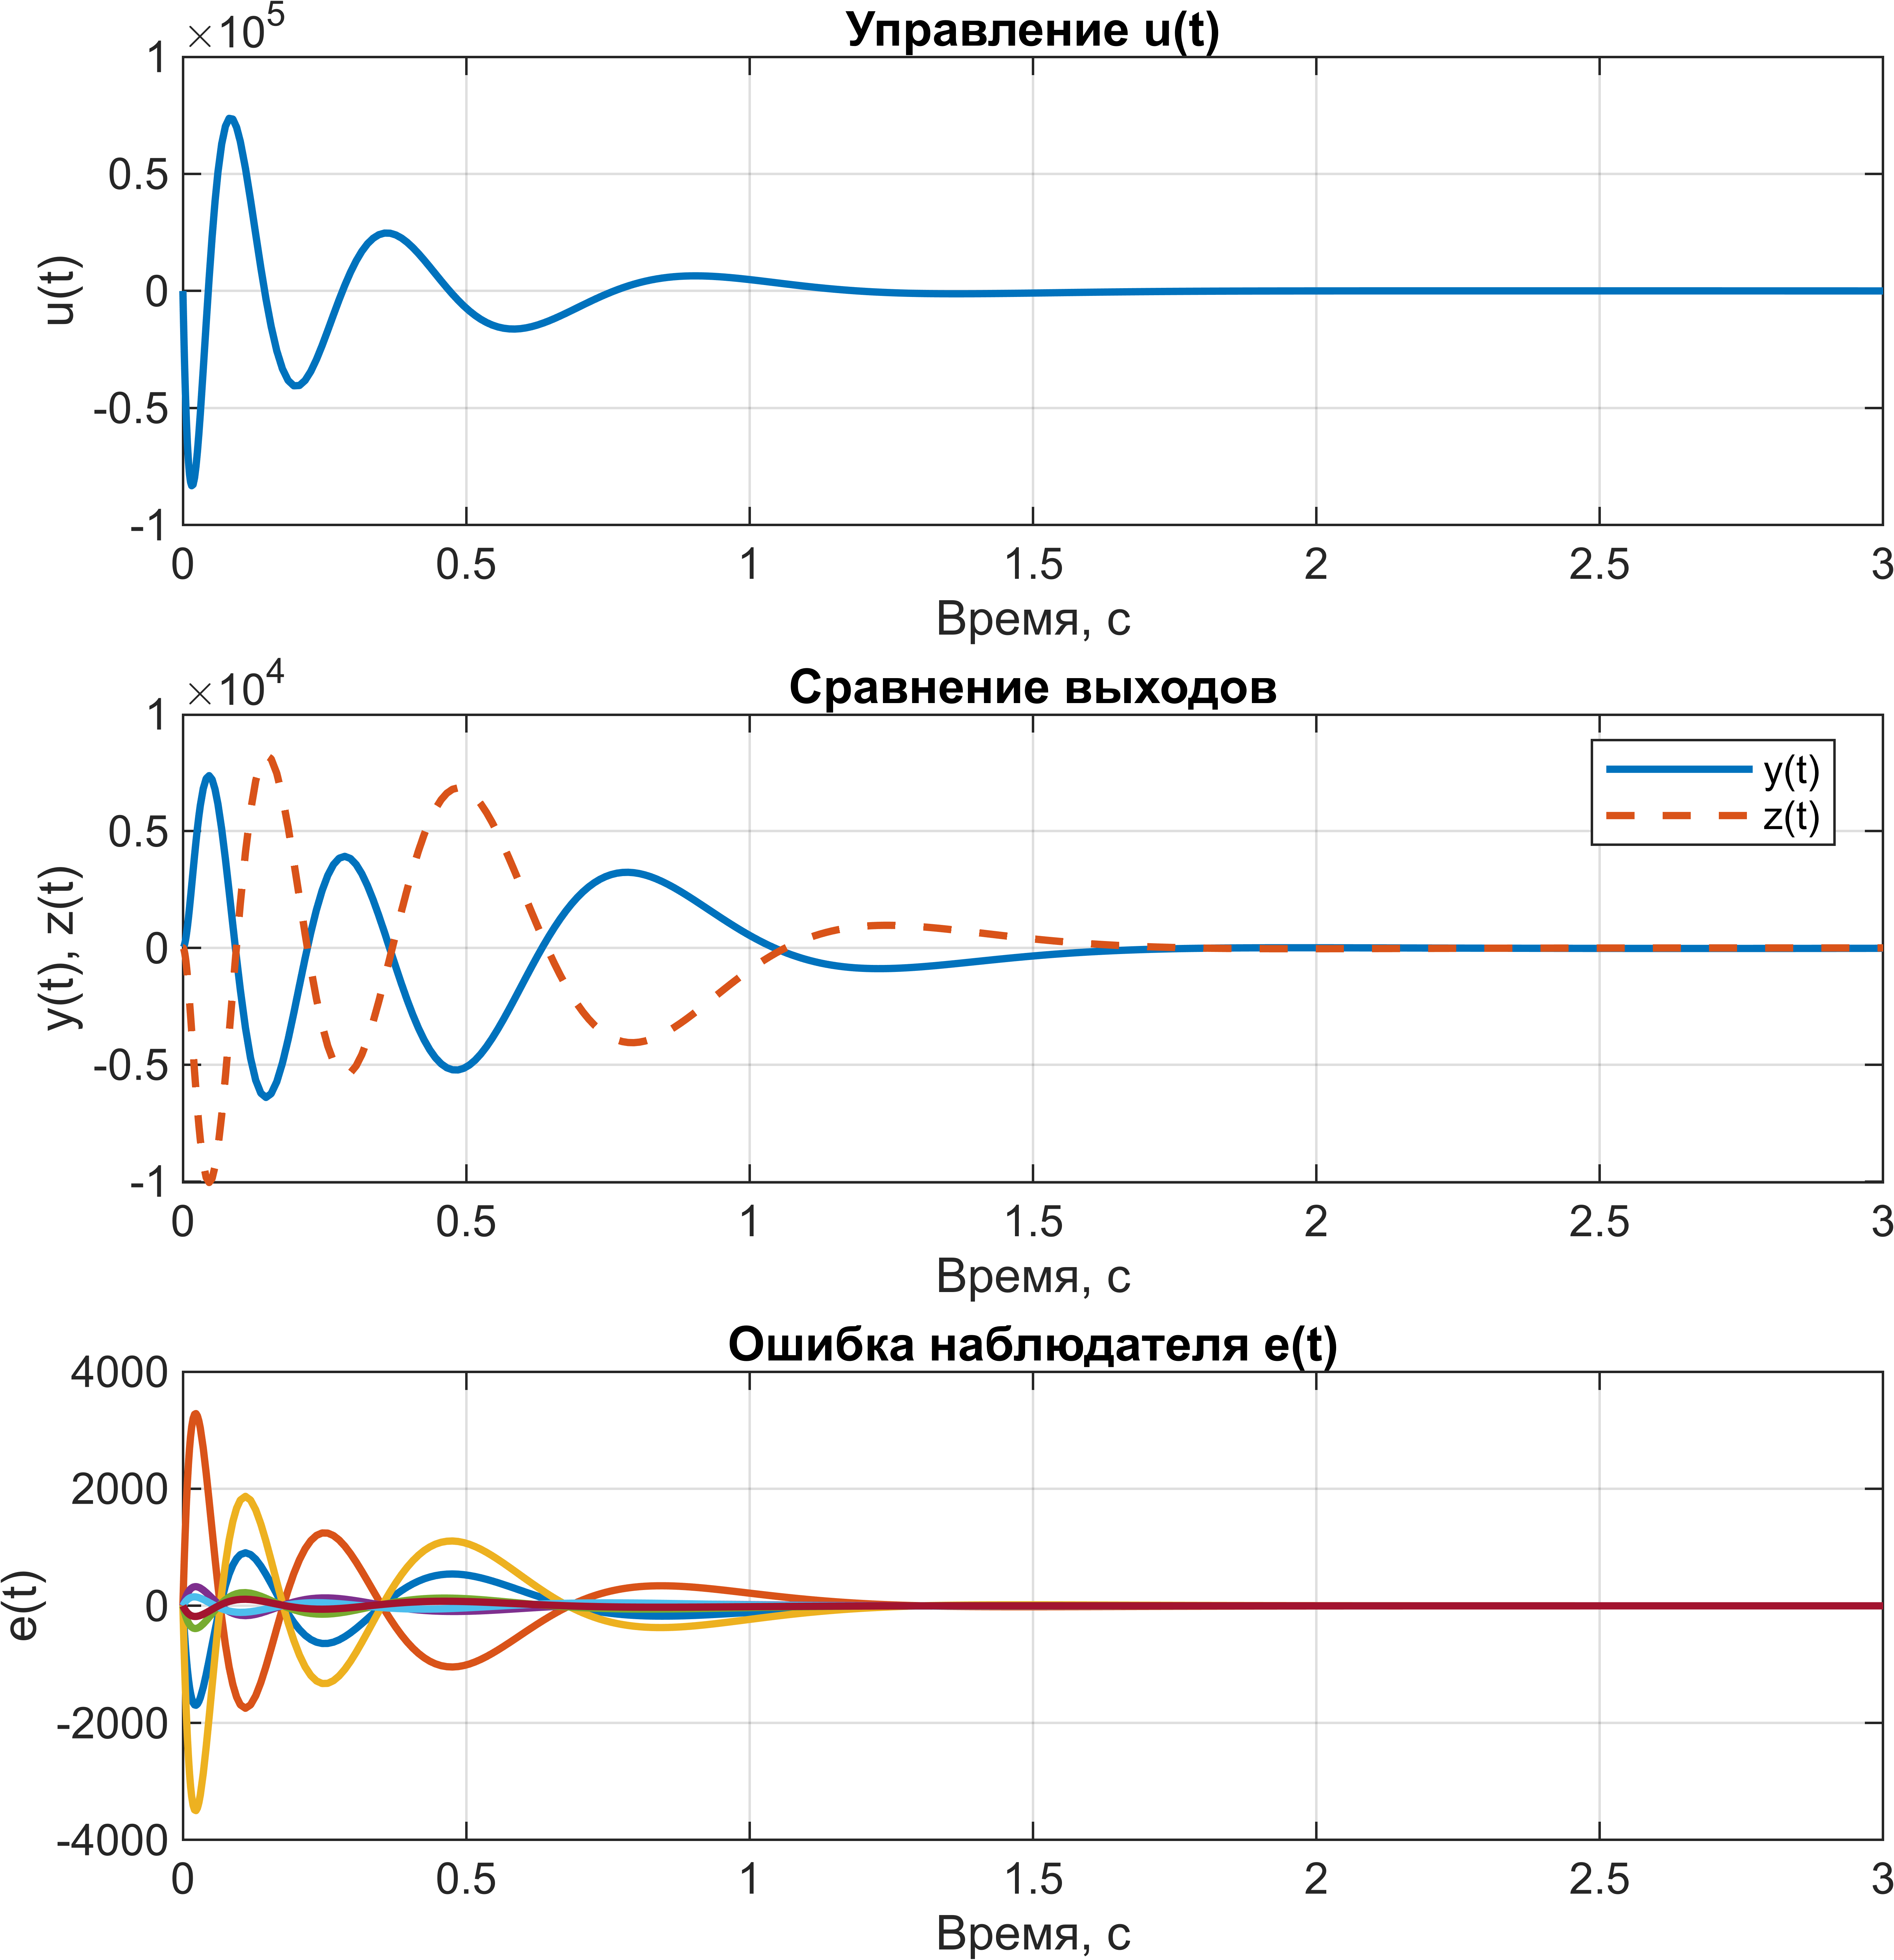
\includegraphics[width=\linewidth]{figs/task3_1.png}
    \caption{Графики управления, ошибуки и выходов}
    \label{fig:3.1}
\end{figure}

\begin{figure}[H]
    \centering
    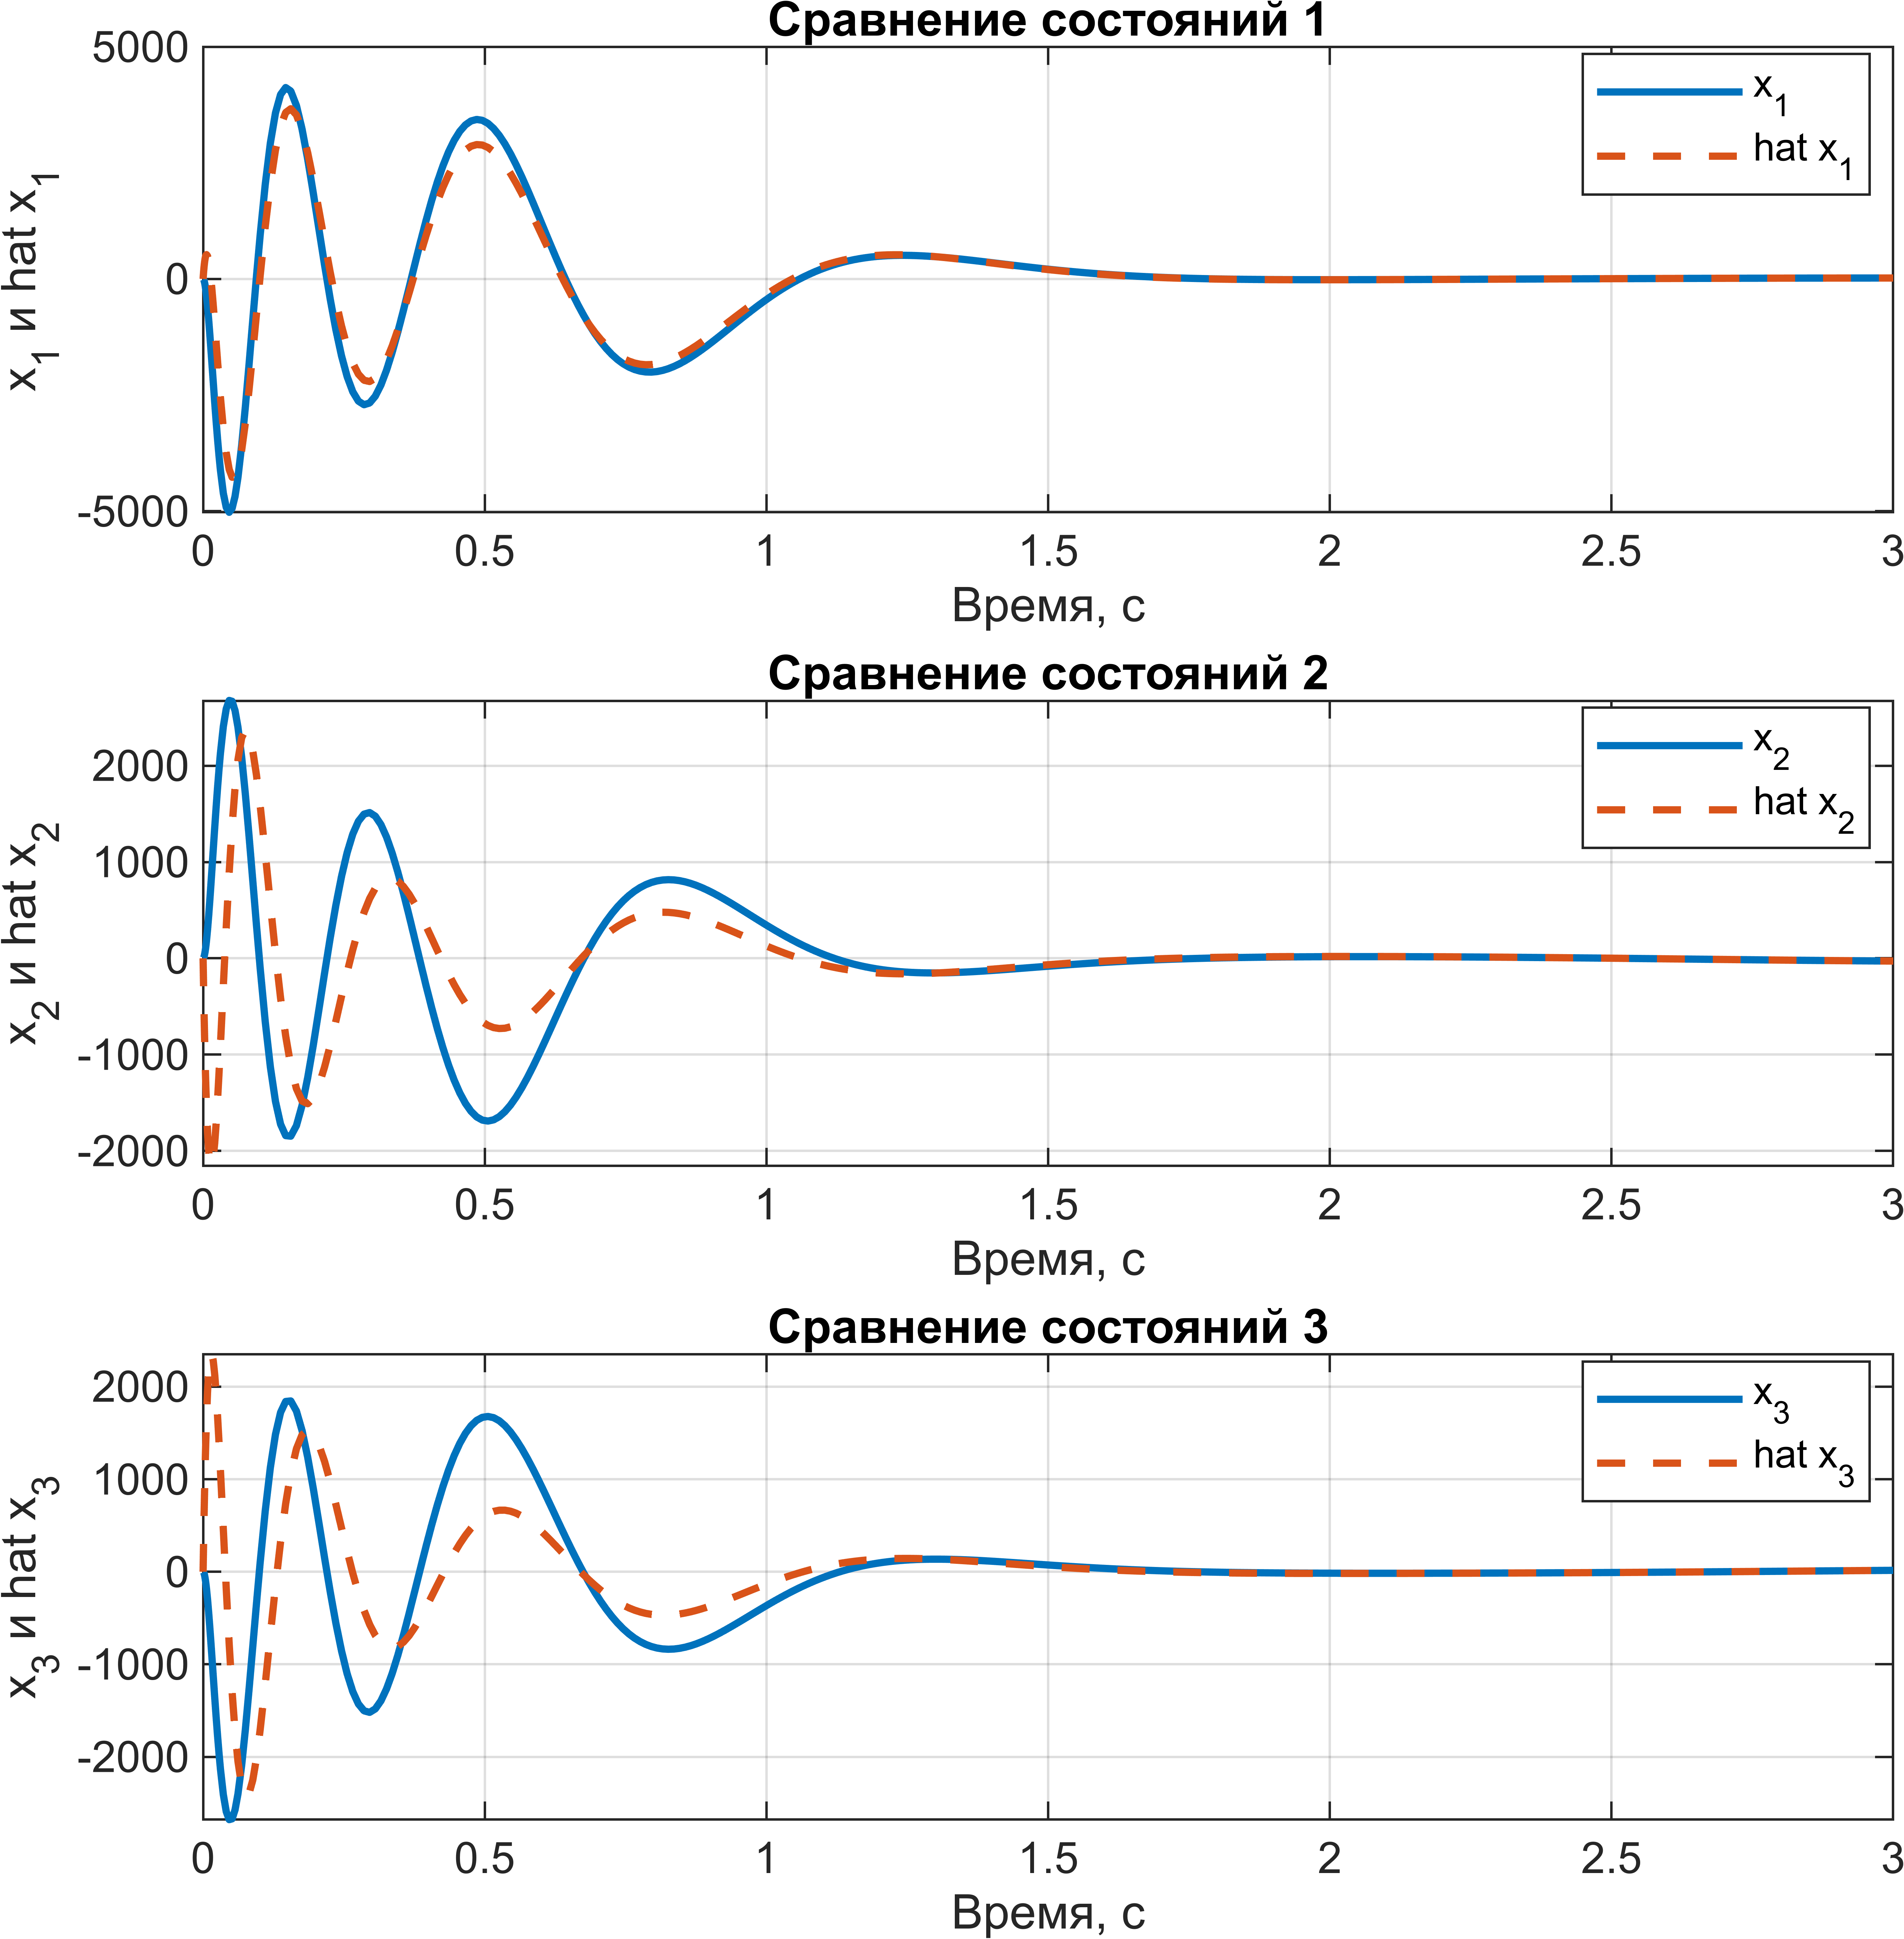
\includegraphics[width=\linewidth]{figs/task3_2.png}
    \caption{Графики состояний}
    \label{fig:3.2}
\end{figure}

\begin{figure}[H]
    \centering
    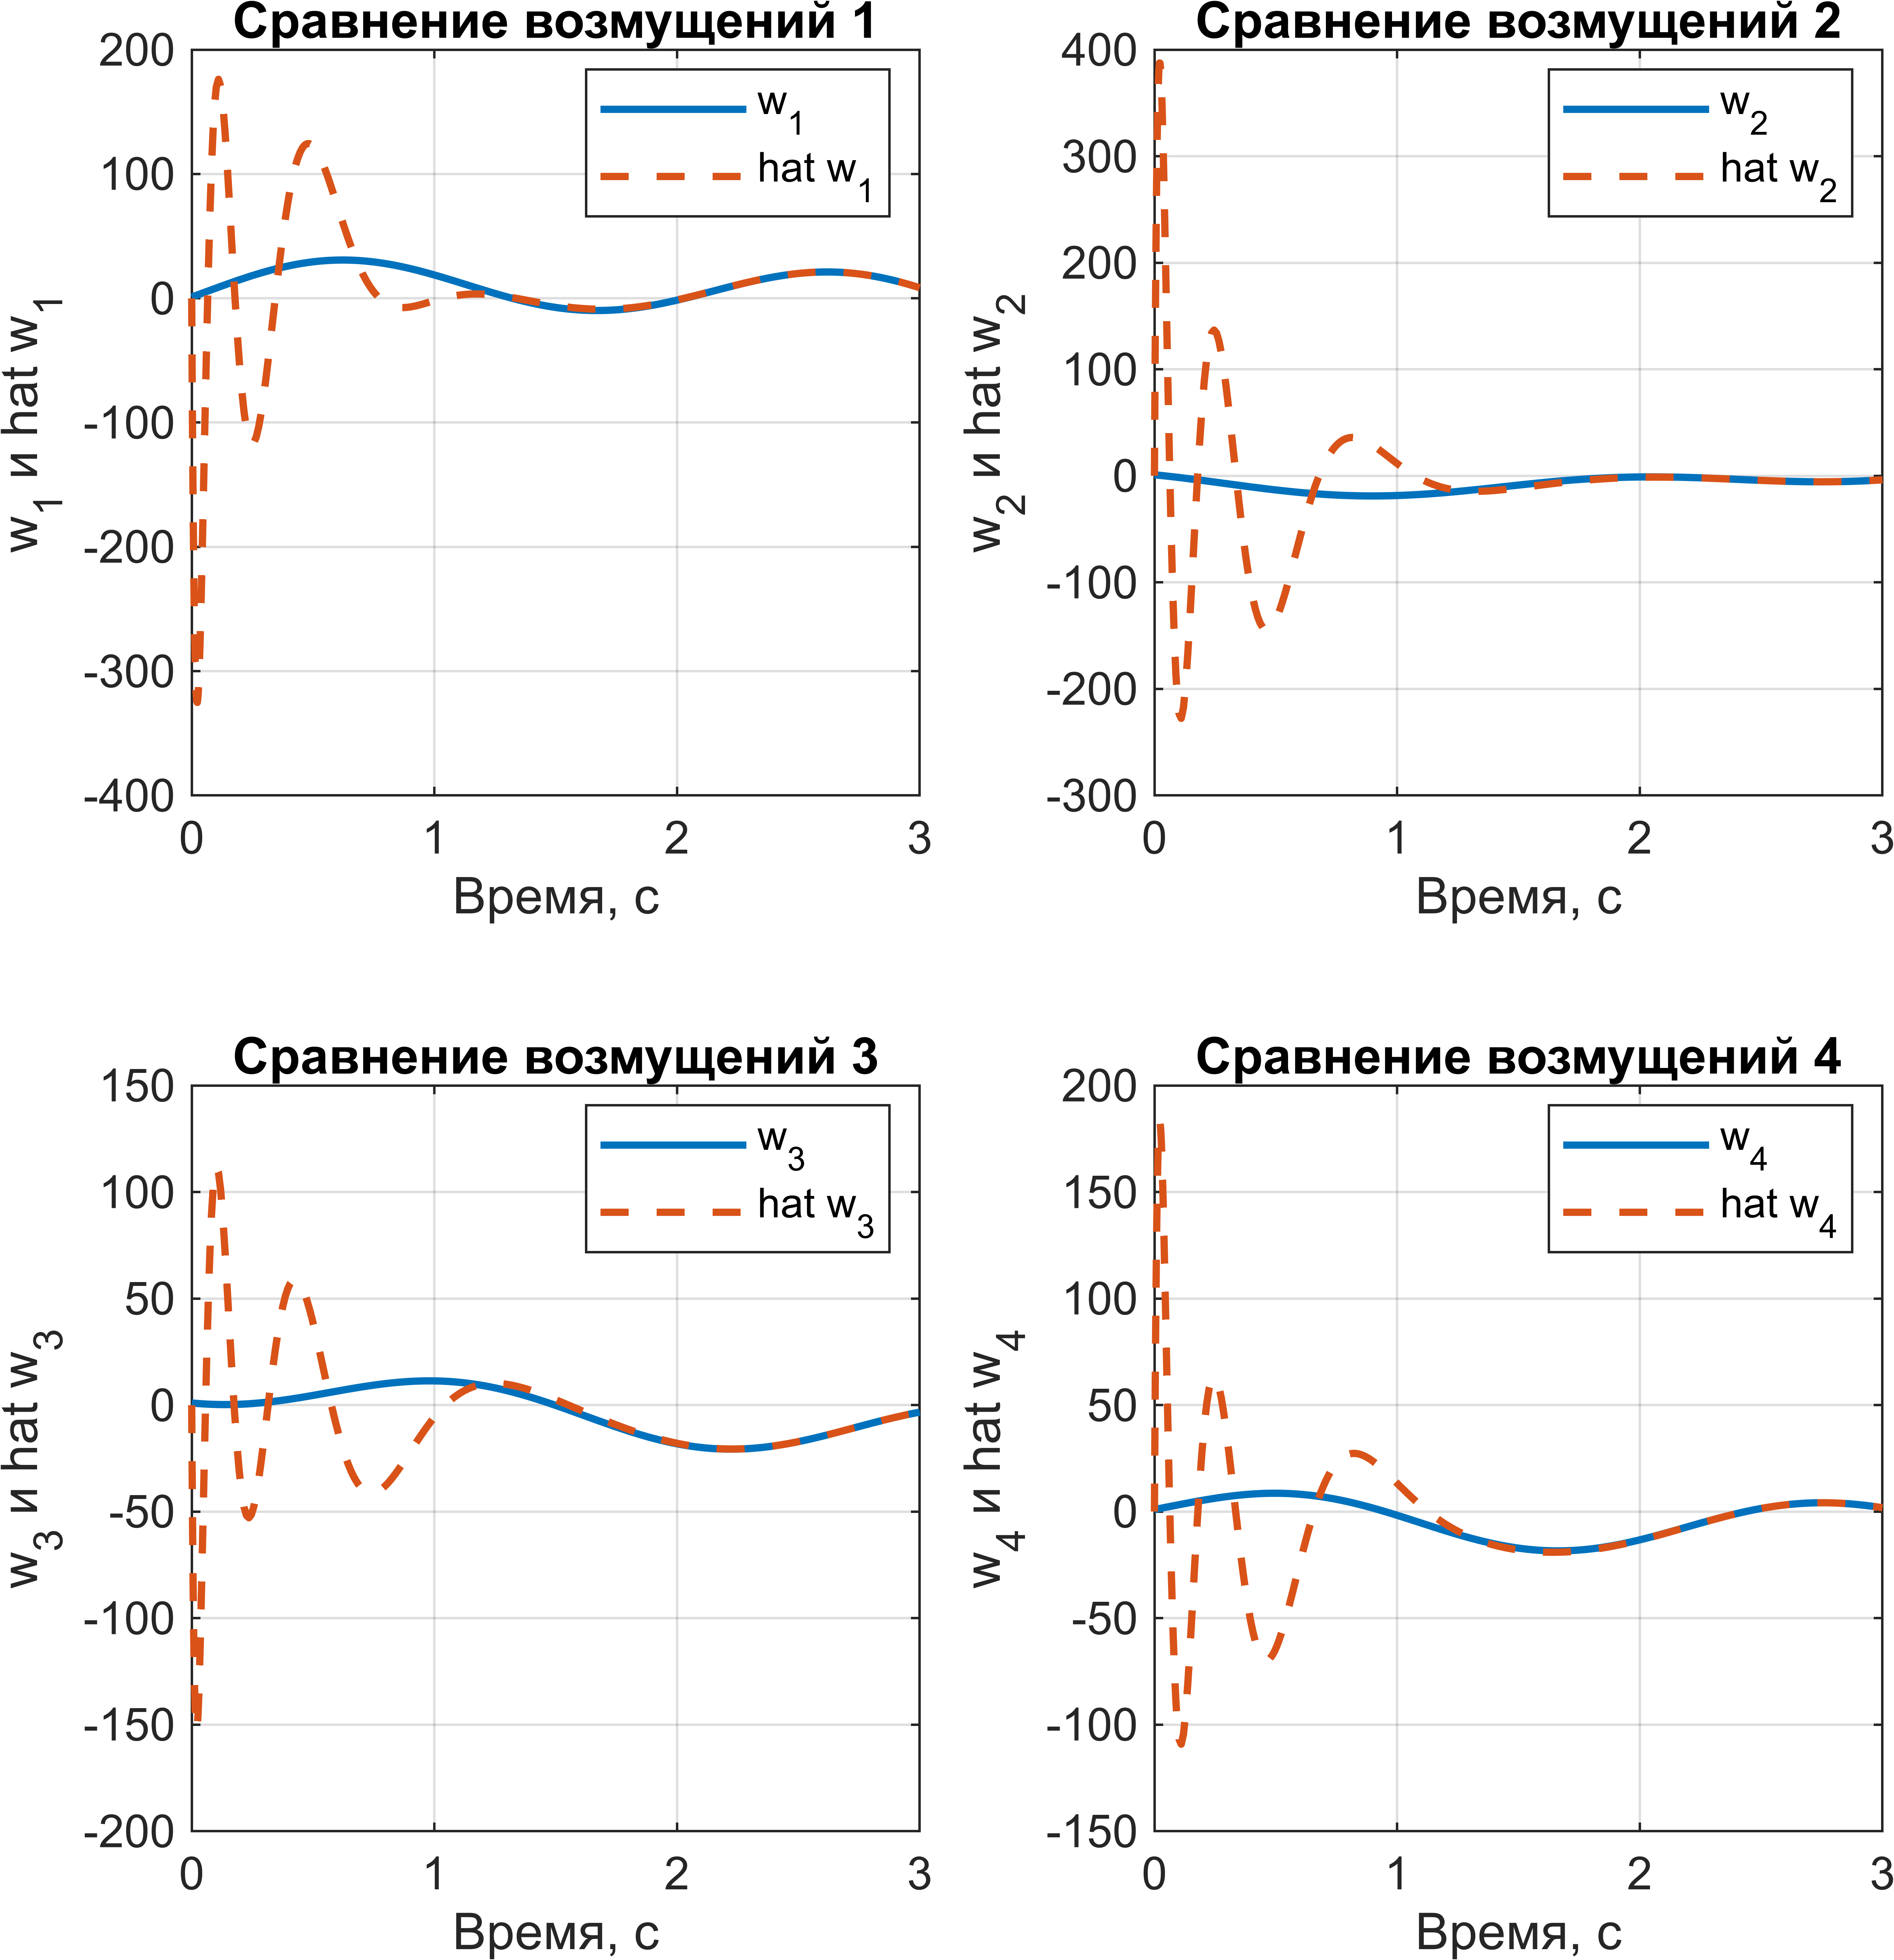
\includegraphics[width=\linewidth]{figs/task3_3.png}
    \caption{Графики возмущения}
    \label{fig:3.3}
\end{figure}


\subsubsection{Другая форма}

Получим уравнения регулятора \eqref{eq:reg3}, \eqref{eq:obs3} в форме ВСВ,
где вход это $y(t)$, а выход $u(t)$:
\begin{equation*}
    \begin{cases}
        \begin{bmatrix}
            \dot{\hat x}\\
            \dot{\hat w}
        \end{bmatrix}=
        \bar A\begin{bmatrix}
            \hat x\\
            \hat w
        \end{bmatrix}-Ly\\
        u=\begin{bmatrix}
            K_1&K_2
        \end{bmatrix}\begin{bmatrix}
            \hat x\\
            \hat w
        \end{bmatrix}
    \end{cases}.
\end{equation*}
Собственные числа матрицы системы $\bar A$ в этой форме следующие
\begin{equation*}
    \sigma(\bar A)=\begin{bmatrix}
            -45.805 \pm 3499.8i \\
            0.0170 \pm 3.0142i \\
            -0.2071 \pm 1.1282i \\
            -2.0109 
    \end{bmatrix}.
\end{equation*}
Сравнивая со спектром матрицы $\Gamma$ \eqref{eq:specG}, можно заметить, что
спектры не пересекаются.






\subsection{Второй случай виртуального выхода}
Рассмотрим виртуальный выход вида:
\begin{equation*}
    z=y.
\end{equation*}

\subsubsection{Синтез ``feedforward''-компоненты}
Аналогично синтезируем «feedforward»-компоненту $K_2$ регулятора \eqref{eq:reg3}.
Получим
\begin{equation*}
    K_2=Y-K_1P=\begin{bmatrix}
        44.7815&	42.7269&	72.1761	&-19.6638
    \end{bmatrix}.
\end{equation*}

\subsubsection{Моделирование}

Выполним компьютерное моделирование замкнутой системы с нулевыми
начальными условиями наблюдателя. График формируемого регулятором 
управления $u(t)$, сравнительные графики
$\begin{bmatrix}
    x(t)\\w(t)
\end{bmatrix}$ и
$\begin{bmatrix}
    \hat x(t)\\\hat w(t)
\end{bmatrix}$, 
график ошибки наблюдателя $e(t)=\begin{bmatrix}
    x(t)\\w(t)
\end{bmatrix} - \begin{bmatrix}
    \hat x(t)\\\hat w(t)
\end{bmatrix}$
и сравнительные графики фактического и виртуального выходов $y(t)$ и $z(t)$
можно увидеть на рисунках \ref{fig:3.4}, \ref{fig:3.5} и \ref{fig:3.6}.
Вируальный выход сошелся к нулю, значит регулятор выпонил своб задачу.

\begin{figure}[H]
    \centering
    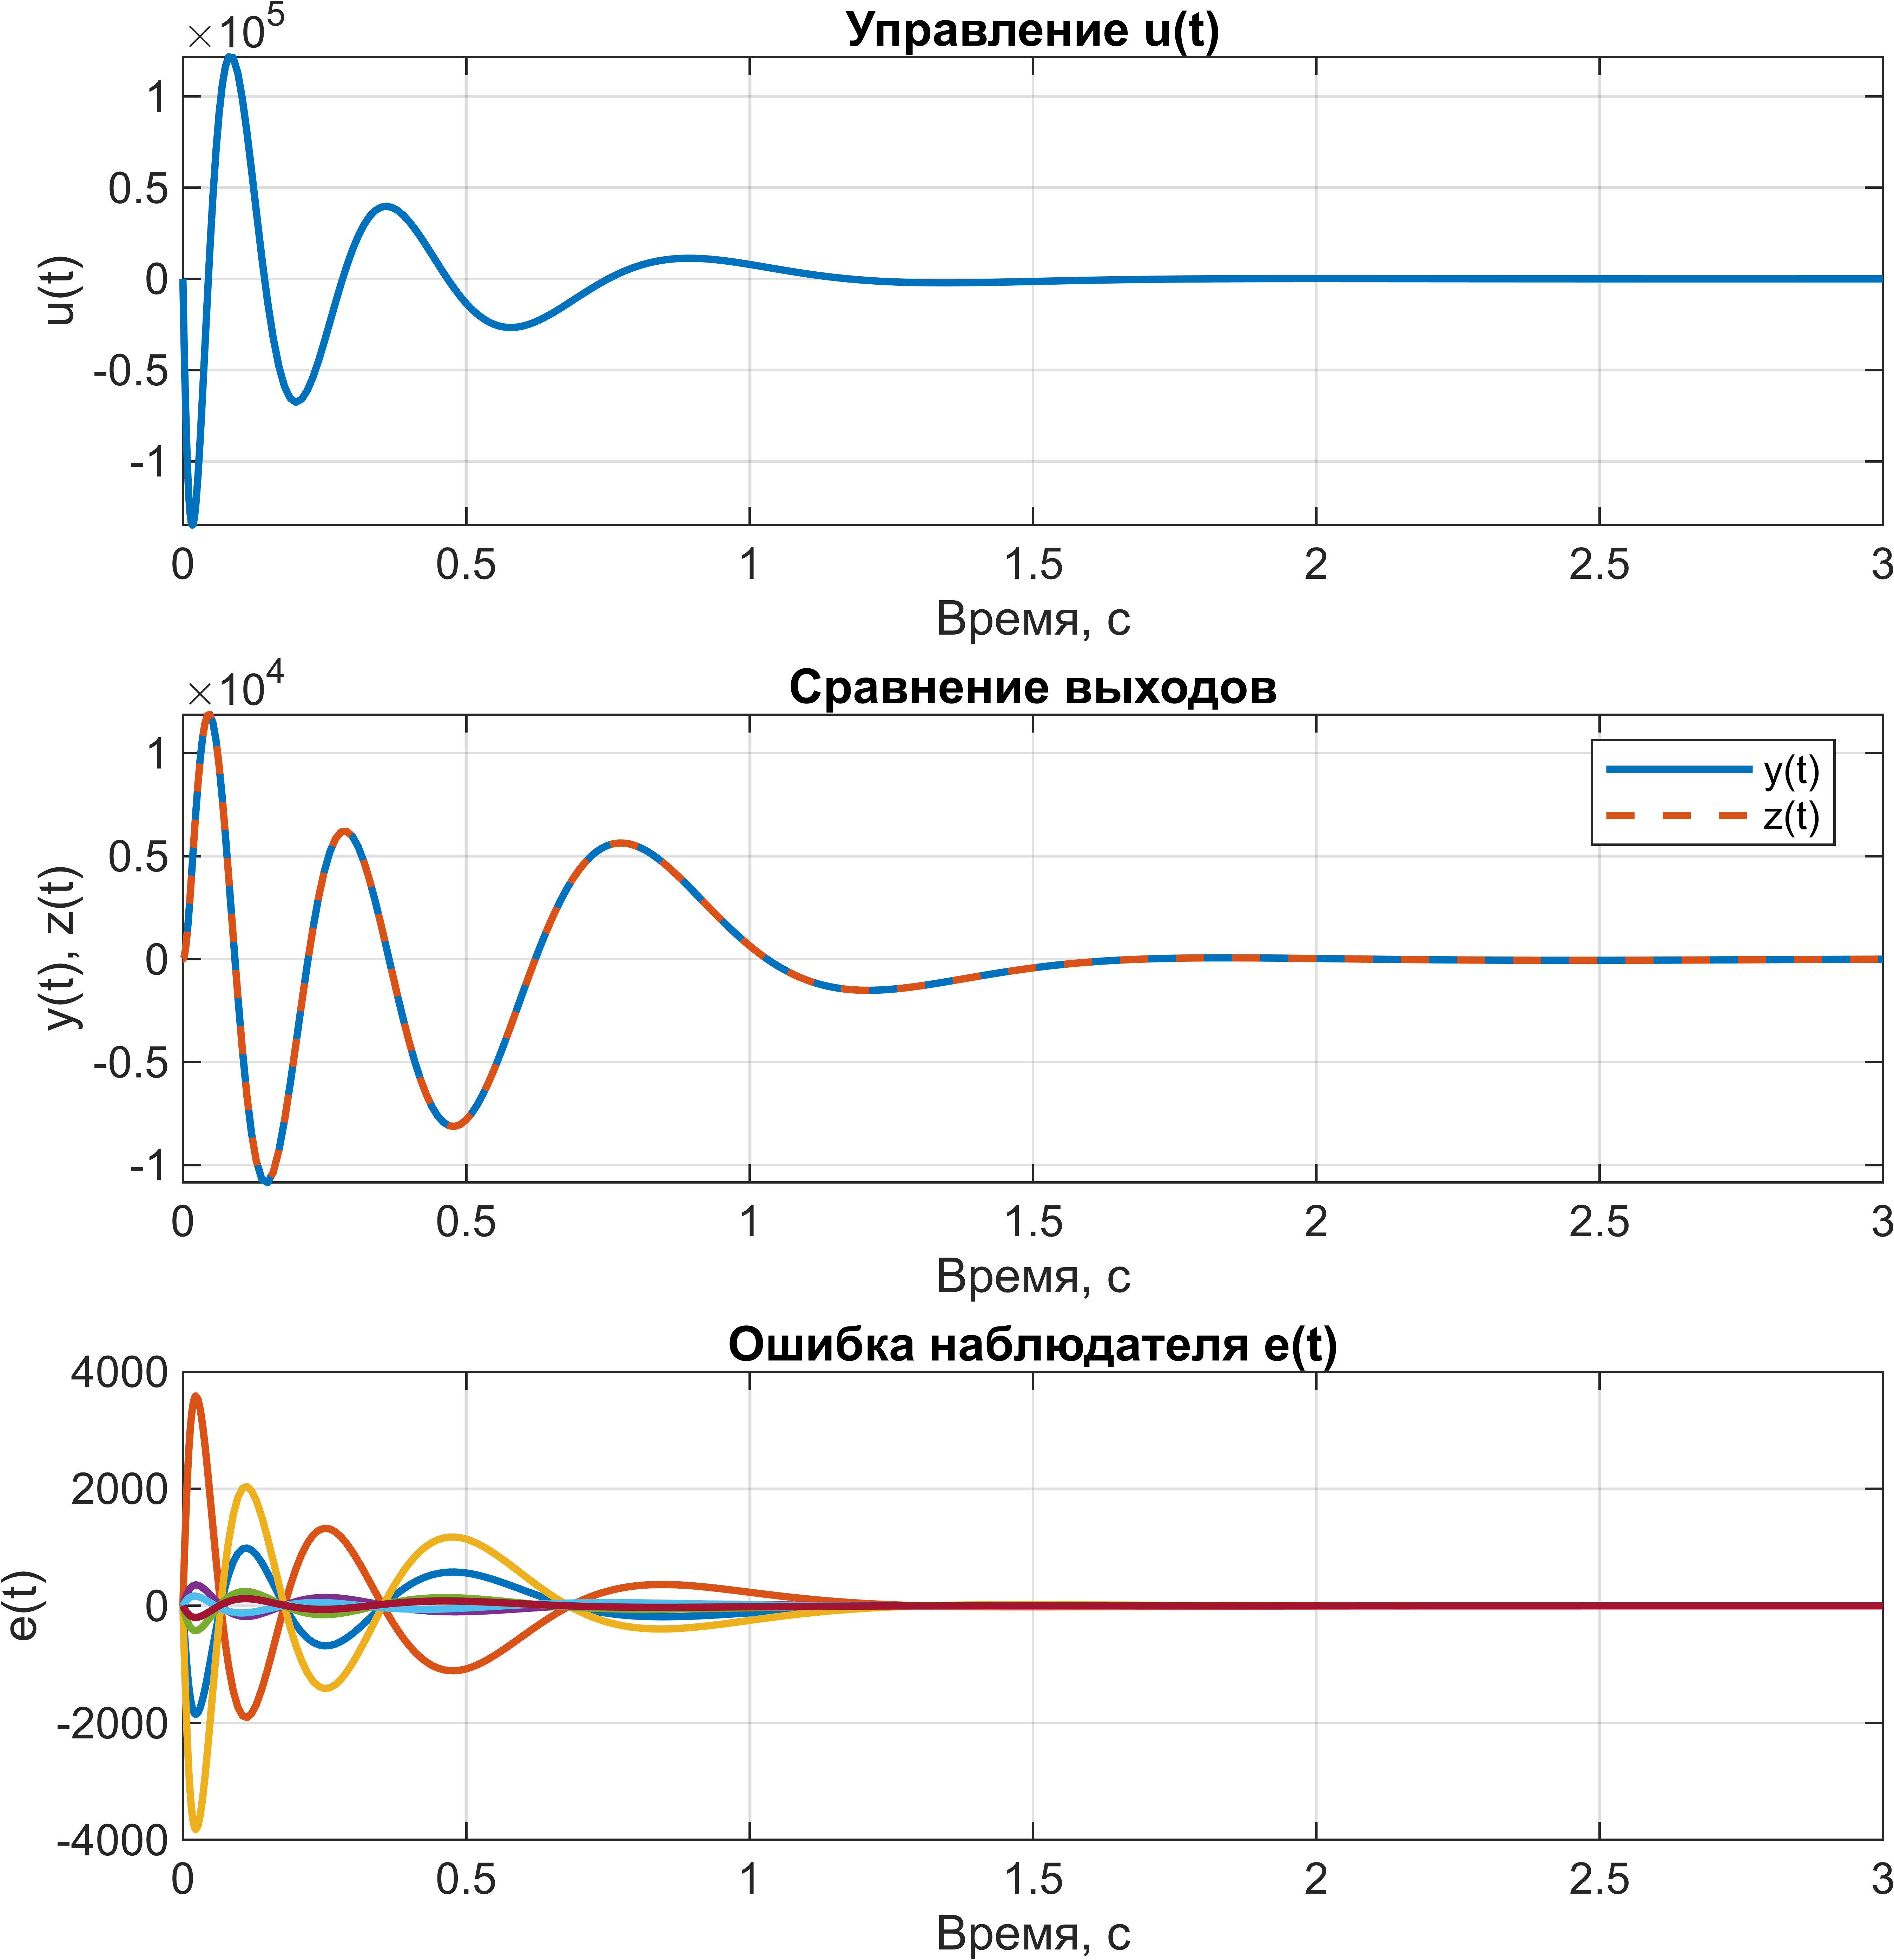
\includegraphics[width=\linewidth]{figs/task3_4.png}
    \caption{Графики управления, ошибуки и выходов}
    \label{fig:3.4}
\end{figure}

\begin{figure}[H]
    \centering
    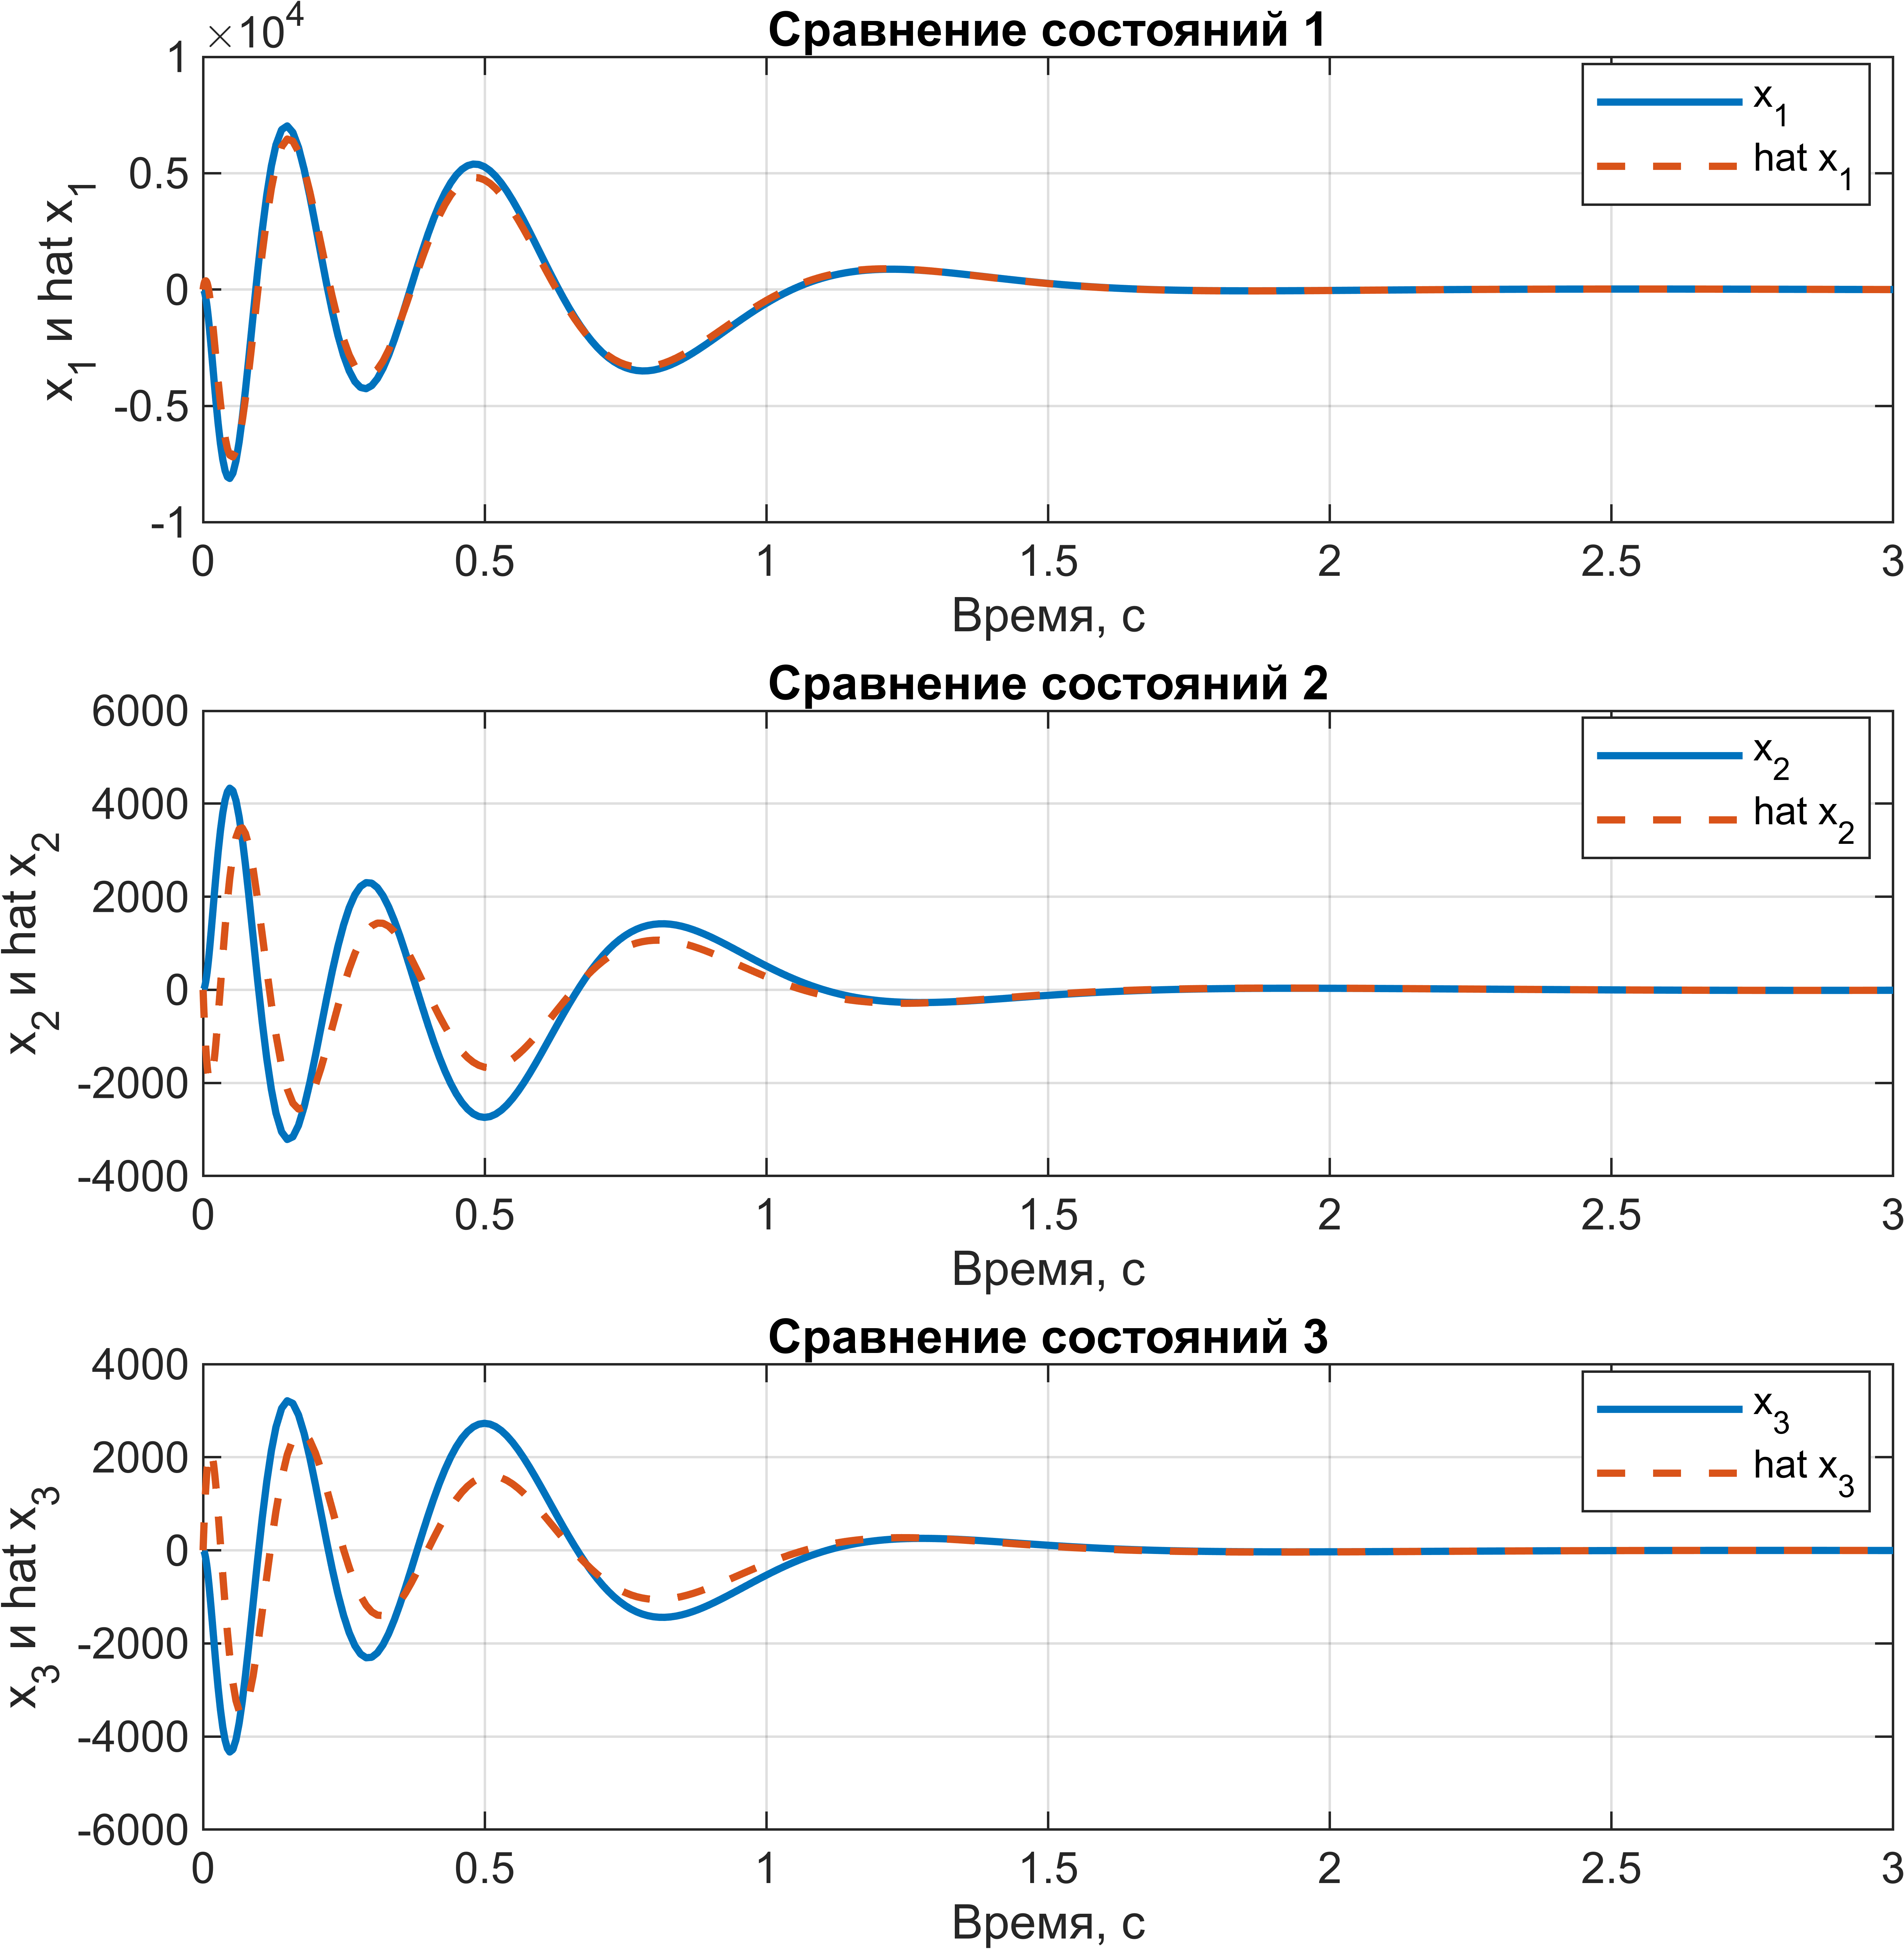
\includegraphics[width=\linewidth]{figs/task3_5.png}
    \caption{Графики состояний}
    \label{fig:3.5}
\end{figure}

\begin{figure}[H]
    \centering
    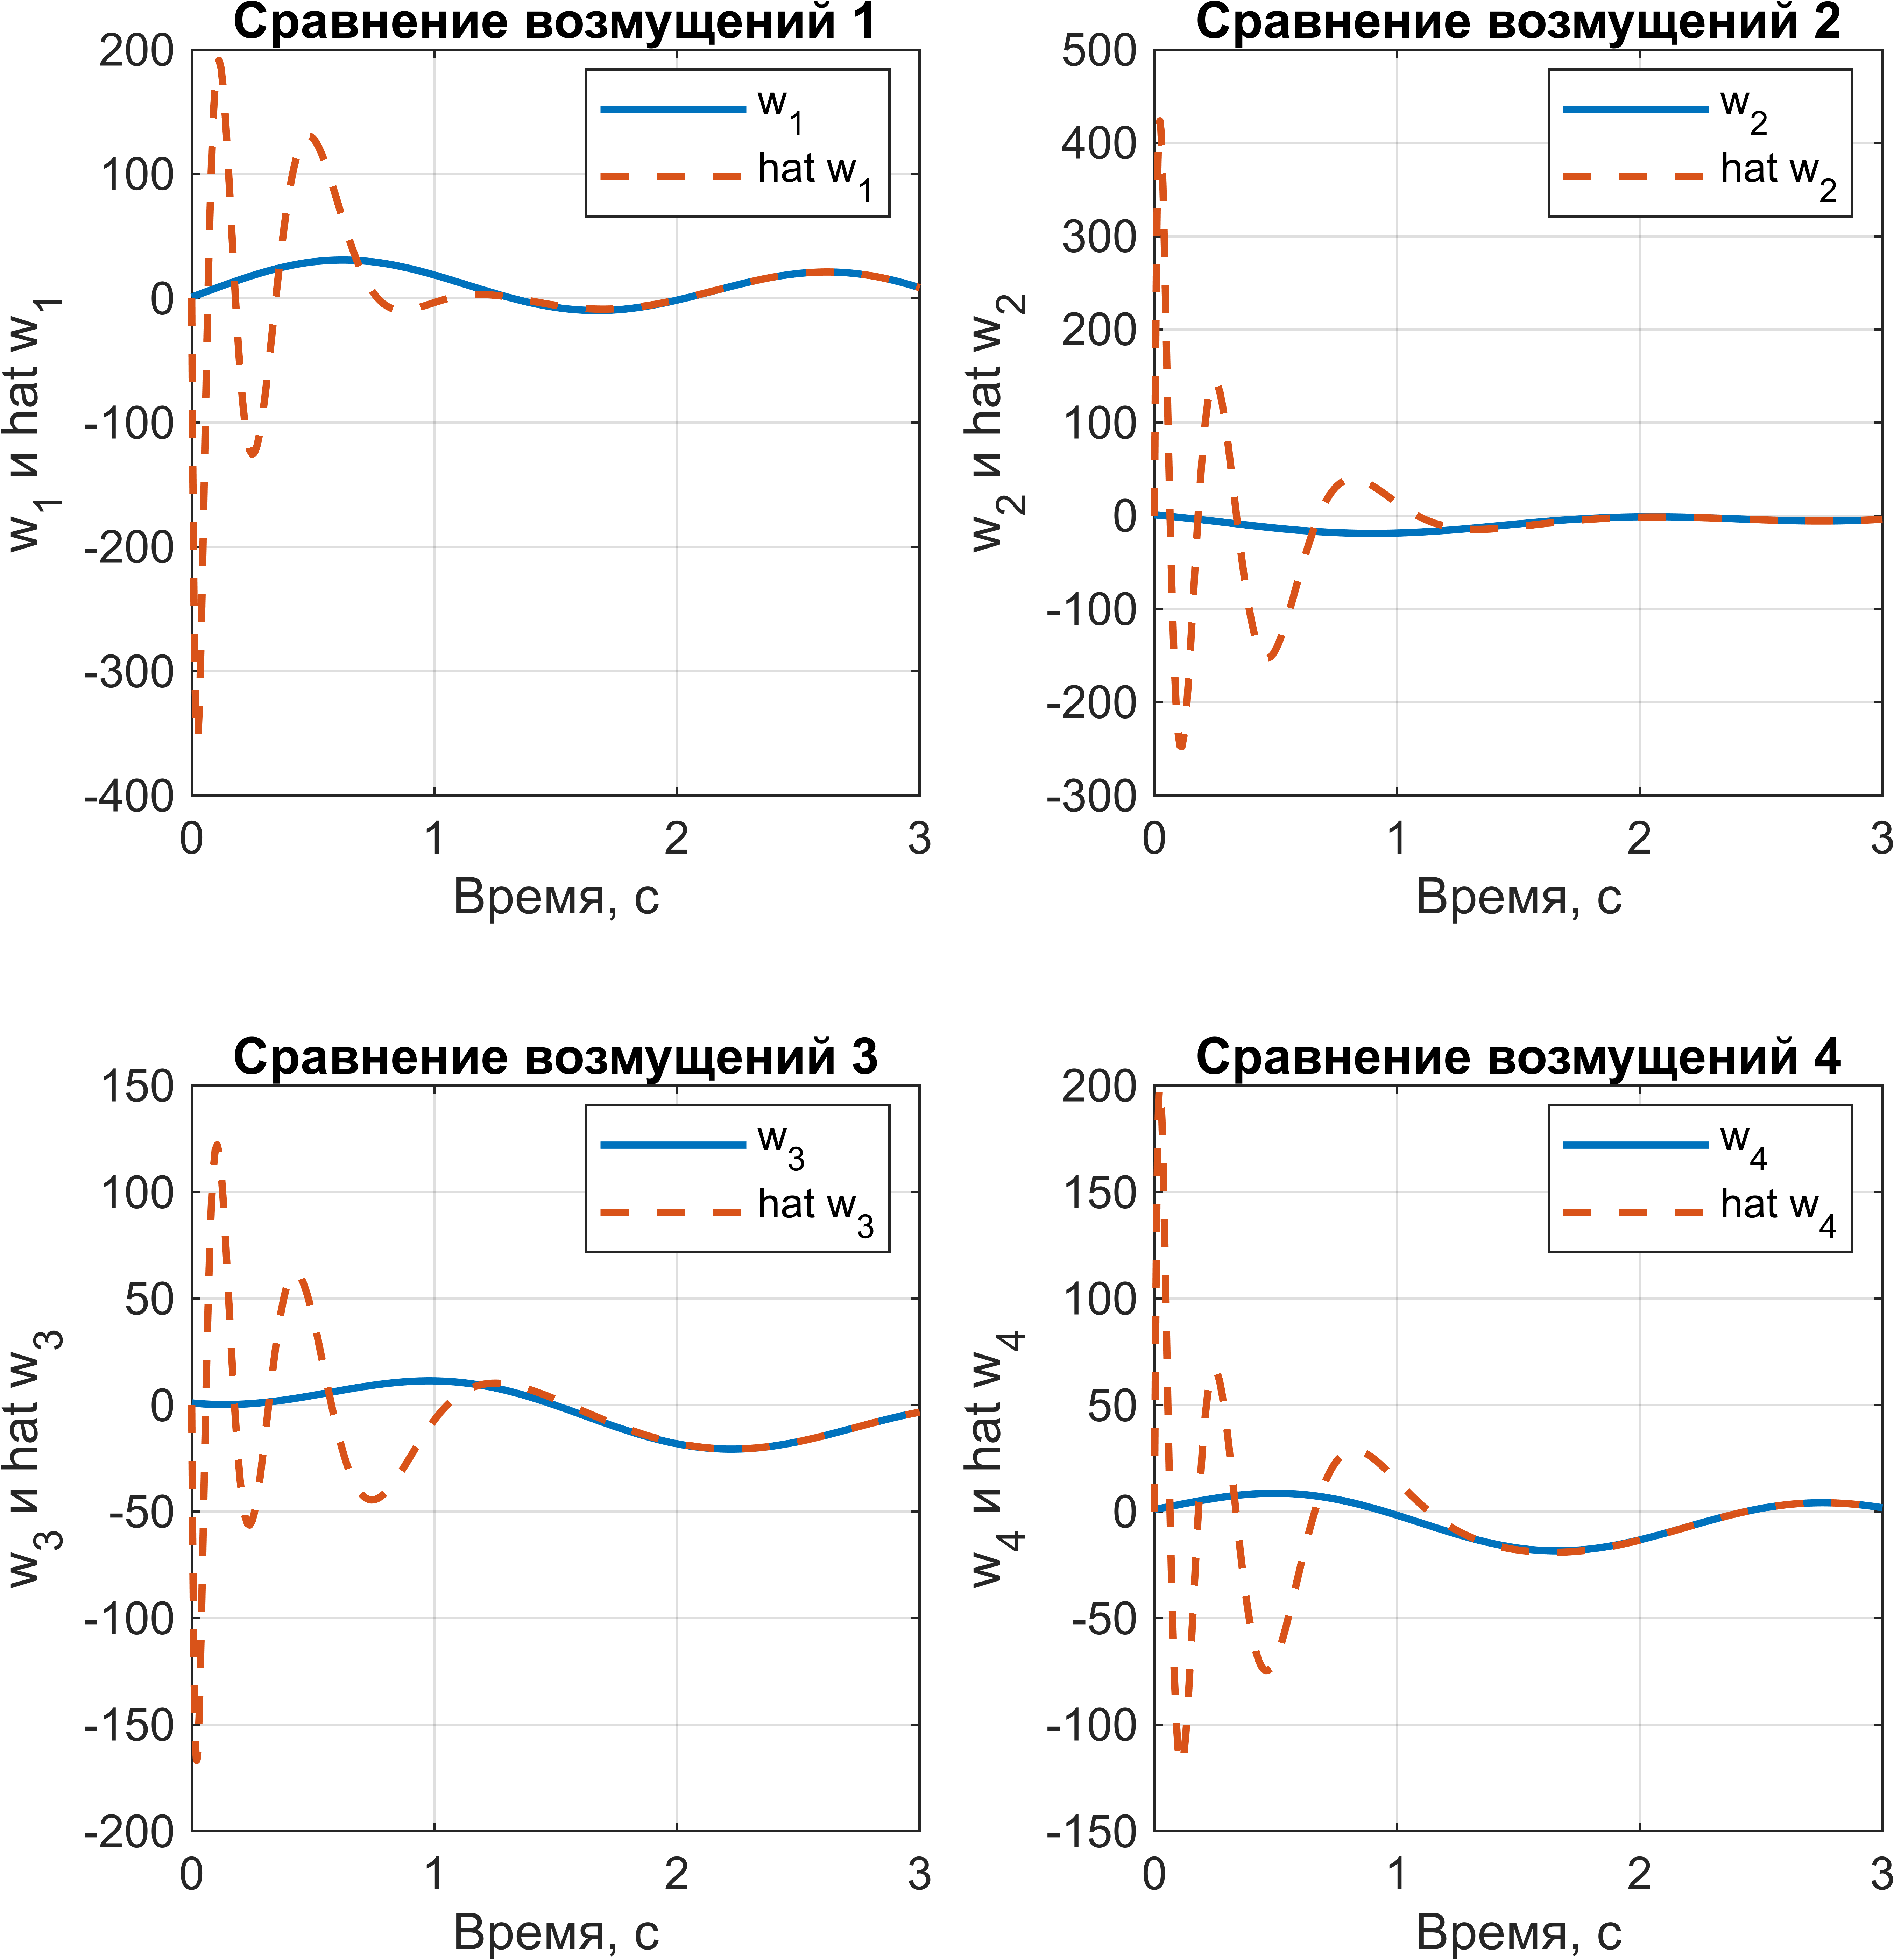
\includegraphics[width=\linewidth]{figs/task3_6.png}
    \caption{Графики возмущения}
    \label{fig:3.6}
\end{figure}


\subsubsection{Другая форма}

В форме ВСВ, где вход это $y(t)$, а выход $u(t)$,
собственные числа матрицы системы в этой форме следующие
\begin{equation*}
    \sigma(\bar A)=\begin{bmatrix}
        -46.275 \pm 4297.9i \\
        -0.0623 \pm 3.0447i \\
        0.3394 \pm 0.9818i \\
        -2.0051
    \end{bmatrix}.
\end{equation*}
Сравнивая со спектром матрицы $\Gamma$ \eqref{eq:specG}, можно заметить, что
спектры не пересекаются, очень похожие собственные числа есть.



\subsection{Вывод}

Был успешно синтезирован регулятор, обеспечивающий слежение и компенсацию 
по выходу, состоящий из ``feedback``- и ``feedforward``-компонент, 
а также расширенного наблюдателя. Регулятор успешно компенсирует внешние возмущения
и выполняет слежение, обеспечивая выполнение целевого условия. В обоих случаях виртуального 
выхода регулятор продемонстрировал корректную работу, спектры системы
регулятора в общем виде (где $y$ вход и $u$ выход) не пересекались со 
спектром генератора возмущений, что мне кажется странным,
так как согласно приципу внутренней модели, в случае $z=y$, спектр матрицы возмущения
должен быть в спектре матрицы системы регулятора в общем виде для успешного
выпонения целевого условия, но есть очень похожие собственные числа, и, видимо,
этого достаточно.




\section{Тележка и меандр}

\begin{figure}[H]
    \centering
    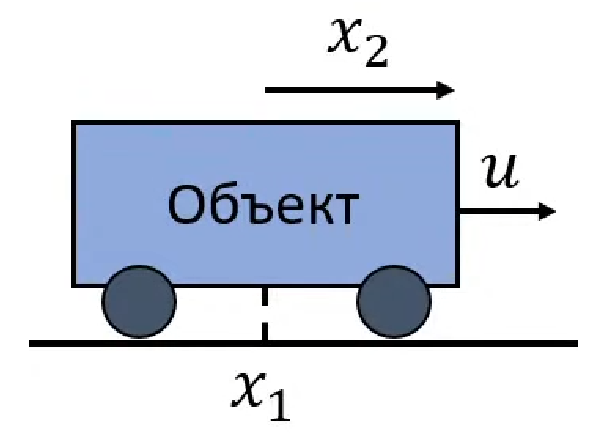
\includegraphics[width=0.4\linewidth]{figs/тележка.png}
    \caption{Тележка}
    \label{fig:cart}
\end{figure}

Рассмотрим объект управления ``тележка'' \autoref{fig:cart}. Синтезируем математическую модель,
приняв в качестве выхода линейную координату $y(t) = x_1(t)$:
\begin{equation*}
    \begin{cases}
        \dot x =Ax+Bu,\\
        y=Cx,
    \end{cases}
\end{equation*}
где
\begin{equation*}
    x=\begin{bmatrix}
        x_1\\x_2
    \end{bmatrix},\quad
    A=\begin{bmatrix}
        0 & 1\\
        0 & 0
    \end{bmatrix},\quad
    B=\begin{bmatrix}
        0\\1
    \end{bmatrix},\quad
    C=\begin{bmatrix}
        1 & 0
    \end{bmatrix}.
\end{equation*}
За задающий сигнал 
примем меандром $g(t)$
\begin{equation}
    g(t) = \begin{cases}
        -a, & t \in [0, T/2)\\
        a, & t \in [T/2, T)
    \end{cases}
\end{equation}
с амплитудой $a=10$ и периодом $T=2\pi$.
Разложим его в ряд Фурье:
\begin{equation*}
    F_m(t)=\frac{a_0}{2}+\sum_{n=1}^{m}(a_n\cos(nt)+b_n\sin(nt)),
\end{equation*}
где
\begin{gather*}
    a_0=\frac{2}{T}\int_0^T g(t)dt,\\
    a_n=\frac{2}{T}\int_0^T g(t)\cos\left(\frac{2\pi nt}{T}\right)dt,\\
    b_n=\frac{2}{T}\int_0^T g(t)\sin\left(\frac{2\pi nt}{T}\right)dt.
\end{gather*}
$a_0$ будет равно нулю, так как интеграл по периуду меандра равен нулю.
$a_n$ также будет равно нулю, так как меандр нечетная функция. Вычислим
$b_n$:
\begin{multline*}
    b_n =\frac{1}{\pi}\int_0^{2\pi}g(t)\sin(nt)dt
    =\frac{a}{\pi n}\left( -\int_{0}^{\pi}\sin(nt)dnt+\int_{\pi}^{2\pi}\sin(nt)dnt \right)\\
    =\frac{a}{\pi n}\left( \cos(nt)\Big|_0^\pi-\cos(nt)\Big|_\pi^{2\pi} \right)
    =\frac{a}{\pi n}(2\cos(\pi n)-\cos(2\pi n)-\cos(0))
    =\frac{2a}{\pi n}[(-1)^n-1].
\end{multline*}
Пусть число гармоник $m=20$, тогда
\begin{multline*}
    \bar g(t)=\frac{20}{\pi}\sum_{n=1}^{20}\frac{(-1)^n-1}{n}\sin(nt) 
    =-\frac{40}{\pi} \big(\sin(t) +\frac{1}{3} \sin(3 t) + \frac{1}{5} \sin(5 t) 
    + \frac{1}{7} \sin(7 t) + \frac{1}{9} \sin(9 t)\\ + \frac{1}{11} \sin(11 t) 
    + \frac{1}{13} \sin(13 t) + \frac{1}{15} \sin(15 t) + \frac{1}{17} \sin(17 t) 
    + \frac{1}{19} \sin(19 t)\big)
\end{multline*}
Сформируем генератор типа
\begin{equation*}
    \dot w=\Gamma w,
\end{equation*}
где
\begin{equation*}
    \Gamma=\begin{bmatrix}
        0  & 1  & 0  & 0  & 0  & 0  & 0  & 0  & 0  & 0  & 0  & 0  & 0  & 0  & 0  & 0  & 0  & 0  & 0  & 0 \\
       -1  & 0  & 0  & 0  & 0  & 0  & 0  & 0  & 0  & 0  & 0  & 0  & 0  & 0  & 0  & 0  & 0  & 0  & 0  & 0 \\
        0  & 0  & 0  & 3  & 0  & 0  & 0  & 0  & 0  & 0  & 0  & 0  & 0  & 0  & 0  & 0  & 0  & 0  & 0  & 0 \\
        0  & 0  &-3  & 0  & 0  & 0  & 0  & 0  & 0  & 0  & 0  & 0  & 0  & 0  & 0  & 0  & 0  & 0  & 0  & 0 \\
        0  & 0  & 0  & 0  & 0  & 5  & 0  & 0  & 0  & 0  & 0  & 0  & 0  & 0  & 0  & 0  & 0  & 0  & 0  & 0 \\
        0  & 0  & 0  & 0  &-5  & 0  & 0  & 0  & 0  & 0  & 0  & 0  & 0  & 0  & 0  & 0  & 0  & 0  & 0  & 0 \\
        0  & 0  & 0  & 0  & 0  & 0  & 0  & 7  & 0  & 0  & 0  & 0  & 0  & 0  & 0  & 0  & 0  & 0  & 0  & 0 \\
        0  & 0  & 0  & 0  & 0  & 0  &-7  & 0  & 0  & 0  & 0  & 0  & 0  & 0  & 0  & 0  & 0  & 0  & 0  & 0 \\
        0  & 0  & 0  & 0  & 0  & 0  & 0  & 0  & 0  & 9  & 0  & 0  & 0  & 0  & 0  & 0  & 0  & 0  & 0  & 0 \\
        0  & 0  & 0  & 0  & 0  & 0  & 0  & 0  &-9  & 0  & 0  & 0  & 0  & 0  & 0  & 0  & 0  & 0  & 0  & 0 \\
        0  & 0  & 0  & 0  & 0  & 0  & 0  & 0  & 0  & 0  & 0  & 11 & 0  & 0  & 0  & 0  & 0  & 0  & 0  & 0 \\
        0  & 0  & 0  & 0  & 0  & 0  & 0  & 0  & 0  & 0  &-11 & 0  & 0  & 0  & 0  & 0  & 0  & 0  & 0  & 0 \\
        0  & 0  & 0  & 0  & 0  & 0  & 0  & 0  & 0  & 0  & 0  & 0  & 0  &13  & 0  & 0  & 0  & 0  & 0  & 0 \\
        0  & 0  & 0  & 0  & 0  & 0  & 0  & 0  & 0  & 0  & 0  & 0  &-13 & 0  & 0  & 0  & 0  & 0  & 0  & 0 \\
        0  & 0  & 0  & 0  & 0  & 0  & 0  & 0  & 0  & 0  & 0  & 0  & 0  & 0  & 0  &15  & 0  & 0  & 0  & 0 \\
        0  & 0  & 0  & 0  & 0  & 0  & 0  & 0  & 0  & 0  & 0  & 0  & 0  & 0  & -15& 0  & 0  & 0  & 0  & 0 \\
        0  & 0  & 0  & 0  & 0  & 0  & 0  & 0  & 0  & 0  & 0  & 0  & 0  & 0  & 0  & 0  & 0  &17  & 0  & 0 \\
        0  & 0  & 0  & 0  & 0  & 0  & 0  & 0  & 0  & 0  & 0  & 0  & 0  & 0  & 0  & 0  &-17 & 0  & 0  & 0 \\
        0  & 0  & 0  & 0  & 0  & 0  & 0  & 0  & 0  & 0  & 0  & 0  & 0  & 0  & 0  & 0  & 0  & 0  & 0  &19 \\
        0  & 0  & 0  & 0  & 0  & 0  & 0  & 0  & 0  & 0  & 0  & 0  & 0  & 0  & 0  & 0  & 0  & 0  &-19 & 0
    \end{bmatrix}.
\end{equation*}
Зададимся виртуальным выходом 
\begin{equation*}
    z=C_Zx+D_Zw,
\end{equation*}
где
\begin{equation*}
    C_Z=\begin{bmatrix}
        -1&0
    \end{bmatrix},\quad
    D_Z=-\frac{40}{\pi}\begin{bmatrix}
        1&0&\frac{1}{3}&0&\frac{1}{5}&0&\frac{1}{7}&0&\frac{1}{9}&0&\frac{1}{11}
        &0&\frac{1}{13}&0&\frac{1}{15}&0&\frac{1}{17}&0&\frac{1}{19}&0
    \end{bmatrix},
\end{equation*}
таким образом, будут выполняться следующие условия:
\begin{equation*}
    \bar g(t)=D_Zw(t),\quad \lim_{t\rightarrow\infty}|\bar g(t)-y(t)|=0.
\end{equation*}

\subsection{Синтез регулятора}
В такой формулировке задача сводится слежению за сигналом $\bar g(t)$.
Синтезируем регулятор вида
\begin{equation*}
    u=K_1x+K_2w.
\end{equation*}
$K_1$ синтезируем с помощью управнения Сильвестра \eqref{eq:silv},
выберем матрицы
\begin{equation*}
    \Gamma_R=\begin{bmatrix}
        -1&	0\\
        0&	-2
    \end{bmatrix},\quad
    Y=\begin{bmatrix}
        1& 1
    \end{bmatrix}
\end{equation*}
и получим:
\begin{equation*}
    K_1=\begin{bmatrix}
        -2&-3
    \end{bmatrix}.
\end{equation*}
$K_2$ синтезируем с помощью уравнений \eqref{eq:getk2}. Получим
\begin{multline*}
    K_2=[
        -12.7324 \quad -38.1972 \quad 29.7089 \quad -38.1972 \quad 58.5690 \quad -38.1972\\ \quad 85.4889 \quad 
        -38.1972 \quad 111.7621 \quad -38.1972 \quad 137.7414 \quad -38.1972 \quad 163.5623 \quad \\-38.1972 \quad 
        189.2883 \quad -38.1972 \quad 214.9528 \quad -38.1972 \quad 240.5753 \quad -38.1972]
\end{multline*}


\subsection{Моделирование}

Выполним компьютерное моделирование, начальное состояние возьмем
нулевое, а начальное состояние возмущения следующее
\begin{equation*}
    w_0=\begin{bmatrix}
        0&1&0&1&0&1&0&1&0&1&0&1&0&1&0&1&0&1&0&1
    \end{bmatrix},
\end{equation*}
убрав косинусы, чтобы генератор повторял $\bar g(t)$.
Графики формируемого регулятором управления $u(t)$,
состояния и сравнение выхода с генерируемым сигналом $\bar g(t)$
можно увидеть на \autoref{fig:cart1}. Тележка успешно следует за
генерируемым сигналом.
\begin{figure}[H]
    \centering
    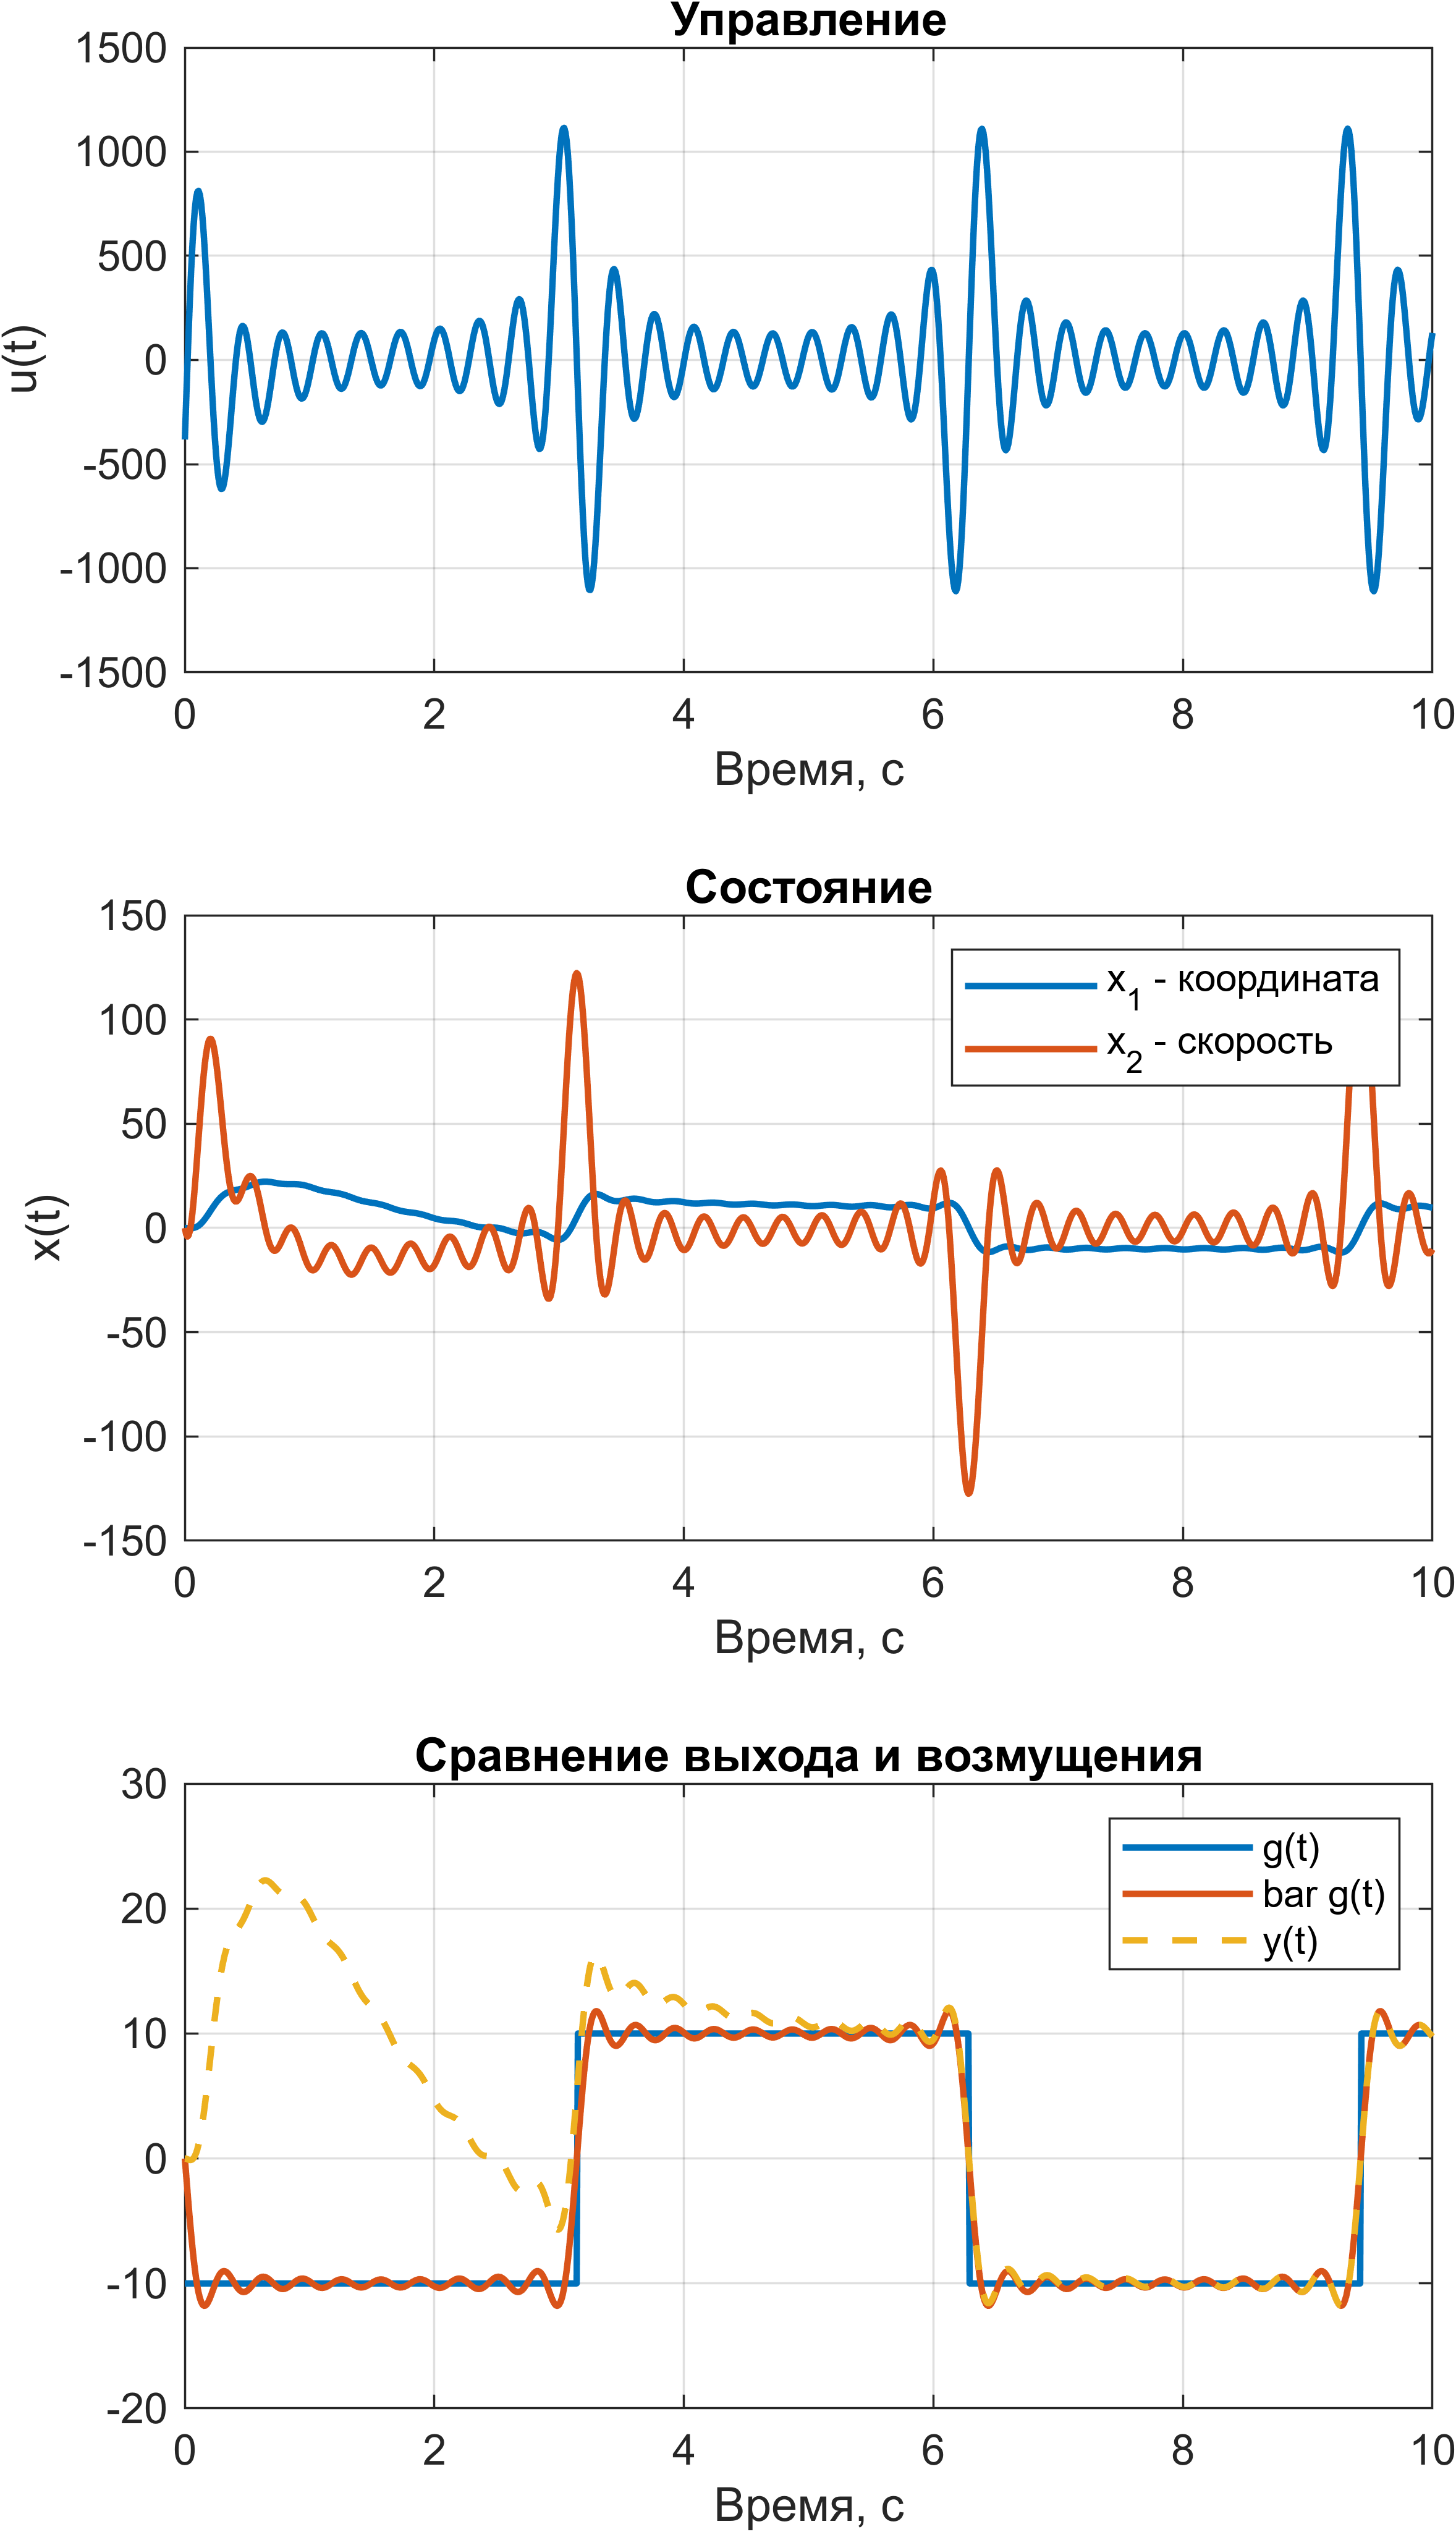
\includegraphics[width=0.8\linewidth]{figs/task4.png}
    \caption{Графики управления, состояния и выхода тележки}
    \label{fig:cart1}
\end{figure}


\subsection{Выводы}

Был успешно синтезирован регулятор тележки, который обеспечивает 
слежение за задающим сигналом в виде меандра. Проведенное моделирование показало, 
что регулятор корректно выполняет свою задачу. 
Достоинства:
\begin{enumerate}
    \item Регулятор выполненяет целевое условие.
    \item Использование генератора возмущений позволяет учитывать 
    периодические сигналы, такие как меандр.
\end{enumerate}
Недостаток:
\begin{enumerate}
    \item Высокая размерность генератора возмущений, при небольшом
    количестве членов ряда Фурье 20, размер матрицы возмущения составляет 400.
\end{enumerate}




\section{Заключение}

В ходе лабораторной работы были успешно синтезированы различные 
регуляторы по состоянию и по выходу: компенсирующий, следящий и регулятор для тележки, 
обеспечивающий слежение за задающим сигналом в виде меандра. 
Проведенное моделирование подтвердило корректность работы всех 
регуляторов, их способность компенсировать внешние возмущения 
и выполнять целевые условия.